    % This is the adapted paper for the LLNCS macro package for Springer
    \documentclass[runningheads]{llncs}

    \usepackage[T1]{fontenc}
    \usepackage{amsmath,amssymb,amsfonts}
    \usepackage{algorithmic}
    \usepackage{graphicx}
    \usepackage{textcomp}
    \usepackage{xcolor}
    \usepackage{booktabs}
    \usepackage{multirow}
    \usepackage{hyperref}
    
    % Professional Academic Styling
    \usepackage{mathptmx} % Times New Roman font (standard for IEEE/Springer)
    \usepackage[margin=1in]{geometry}
    \usepackage{microtype} % Improves typography and justification

    \begin{document}

    \title{Quantifying Institutional Liquidity Sweeps: Tail-Risk Protection via Deep Temporal Architectures in Emerging Markets}

    \titlerunning{Quantifying Institutional Liquidity Sweeps}

    \author{Thien Khoi Nguyen\inst{1}\orcidID{0009-0006-8652-6493},
    Thu Le\inst{2}\orcidID{0009-0008-3480-8311}, \\
    Minh Triet Nguyen\inst{3}\orcidID{0009-0001-0680-7433}, \\
    Hung Anh Tran\inst{4}\orcidID{0009-0008-9452-1582}, \and
    Viet Hoang Van\inst{5}\orcidID{0009-0005-5905-2598}}

    \authorrunning{N. T. Khôi}

    \institute{FPT University, Ho Chi Minh Campus, Vietnam \\
    \email{nguyenthienkhoi0403@gmail.com, thulvm@fe.edu.vn, \\
    \{nguyenntriett, tranhunganhstark152, vanviethoang2000\}@gmail.com}}

    \maketitle

    \begin{abstract}
    Retail investors in emerging markets are frequently disadvantaged by institutional stop-hunting mechanisms, falling victim to liquidity traps driven by distinct market structures. To address these systemic disparities, we propose a mathematically formalized quantitative trading framework that shifts from traditional technical indicators to a pure price-action quantification of Smart Money Concepts (SMC). Specifically, we mathematically model ``Liquidity Sweep'' patterns---comprising both bullish and bearish variants---utilizing atomic OHLCV data to detect institutional intervention. To identify the optimal algorithmic core capable of providing tail-risk protection during market crashes, we empirically evaluate four deep temporal architectures across three Market Regimes (Stable, Normal, Extreme) using Vietnam's VN30 index as a preliminary proxy for frontier emerging-market liquidity profiles \cite{bekaert1995time}. Experimental results demonstrate that LSTM demonstrates potential for outperforming competing architectures during Extreme Regimes, with an out-of-sample Sharpe Ratio of 1.06 on the VN30 test partition. The winning recursive model is deployed as a proof-of-concept system, providing transaction-cost-adjusted Action Scores to illustrate potential practical viability for retail traders. Generalization to other emerging markets remains an open research question.

    \keywords{Quantitative Finance \and Smart Money Concepts \and Pure Price-Action \and Emerging Markets \and Time Series Forecasting.}
    \end{abstract}

    \section{Introduction}
    Retail trading is traditionally burdened by emotional biases, impulsive decision-making, and the psychological fatigue associated with continuous tape reading. Furthermore, individual investors operate under significant systemic disadvantages, routinely falling victim to stop-hunts and liquidity shakeouts strategically orchestrated by institutional participants. This dynamic is particularly pronounced in frontier emerging markets, where liquidity profiles are distinct and institutional footprint impacts are highly asymmetric \cite{kyle1985continuous}\cite{amihud2002illiquidity}. While conventional algorithmic trading mitigates some emotional fatigue, it frequently relies on lagging technical indicators (e.g., Moving Averages, RSI) that generate false signals during sophisticated institutional manipulations \cite{pring2002technical}.

    In recent years, Smart Money Concepts (SMC) have emerged as a practitioner paradigm to interpret market microstructure mechanics. SMC focuses on structural elements such as order block formations, fair value gaps, and, crucially, liquidity sweeps. Despite its practitioner efficacy, SMC remains largely a discretionary framework with limited formal mathematical treatment. Integrating SMC with pure price-action quantitative algorithms represents a largely unexploited frontier in FinTech research.

    Recent comprehensive reviews of machine learning and deep learning techniques in stock market prediction highlight several critical open challenges. Most notably, current models struggle with extreme financial noise, lack of interpretability, and severe vulnerability to sudden market regime shifts or ``Black Swan'' events \cite{mdpi2024review}. Regime-switching behavior in financial markets has been studied extensively through hidden Markov models and Markov-switching frameworks \cite{hamilton1989new}\cite{guidolin2011markov}, yet their integration with deep learning architectures for tail-risk-specific feature engineering remains underexplored. Furthermore, standard predictive architectures often fail to account for real-world transaction costs \cite{almgren2001optimal}, rendering them ineffective in practical trading environments.

    \paragraph{Related Work.}
    The literature on institutional market microstructure \cite{kyle1985continuous}\cite{glosten1985bid} establishes that informed participants systematically exploit retail stop-loss clustering, creating predictable price-impact patterns. Within the machine learning literature, recurrent architectures such as LSTM \cite{hochreiter1997} have demonstrated strong performance on financial time series \cite{fischer2018deep}, while attention-based Transformers \cite{vaswani2017} have achieved state-of-the-art results in high-frequency settings \cite{nie2022patchtst}\cite{li2024itransformer}. However, the specific intersection of quantified SMC features and regime-conditioned deep learning for emerging frontier markets---where data scarcity exacerbates overfitting risk---has received no formal academic treatment to our knowledge. This gap motivates the present study.

    While the broader SMC framework encompasses multiple market structures---such as Break of Structure (BOS), Change of Character (CHoCH), and Order Blocks (OB)---this study intentionally isolates and mathematically models the Liquidity Sweep as a first formalization step. Liquidity Sweeps represent a high-conviction institutional manipulation tactic, exhibiting a clear and deterministic price signature (pierce followed by reversal with anomalous volume), which makes them uniquely tractable for mathematical formalization. The exclusion of Order Blocks and CHoCH from the quantitative tensor is acknowledged as a limitation; their integration is reserved for future work.

    This preliminary investigation is evaluated exclusively on Vietnam's VN30 index, which serves as a proxy for frontier emerging-market liquidity profiles. The resulting framework culminates in a proof-of-concept deployment providing transaction-cost-adjusted Action Scores, demonstrating potential practical viability for retail traders.

    \section{Methodology \& Feature Engineering}

    \subsection{Quantifying Smart Money Concepts: Liquidity Sweeps}
    The central premise of our feature engineering pipeline is that major directional moves are preceded by liquidity sweeps---instances where price deliberately pierces structural boundaries to trigger retail stop-loss orders before aggressively reversing \cite{kyle1985continuous}.

    We mathematically model Liquidity Sweeps utilizing atomic OHLCV (Open, High, Low, Close, Volume) data. Let $L_t$ denote the local Swing Low over a historical rolling window of $w$ periods:
    \begin{equation}
    L_t = \min_{i=t-w}^{t-1} (\text{Low}_i)
    \end{equation}

    The window $w = 20$ is selected to represent one calendar trading month of structural context---the canonical practitioner definition of a short-term swing structure---providing sufficient historical depth to identify meaningful support/resistance without introducing excessive look-back bias \cite{lo2000foundations}.

    Similarly, the moving average of the trading volume $\mu_{V,t}$ is defined as:
    \begin{equation}
    \mu_{V,t} = \frac{1}{w} \sum_{i=t-w}^{t-1} \text{Volume}_i
    \end{equation}

    \paragraph{Bullish Liquidity Sweep.}
    A bullish sweep ($LS_t^{+}$) is flagged if price action temporarily violates $L_t$ but subsequently mean-reverts to close above it, accompanied by anomalous volume:
    \begin{equation}
    LS_t^{+} = \begin{cases} 1, & \text{if } \text{Low}_t < L_t \land \text{Close}_t > L_t \land \text{Volume}_t > k \cdot \mu_{V,t} \\ 0, & \text{otherwise} \end{cases}
    \end{equation}

    \paragraph{Bearish Liquidity Sweep.}
    Symmetrically, let $H_t$ denote the local Swing High over the same window:
    \begin{equation}
    H_t = \max_{i=t-w}^{t-1} (\text{High}_i)
    \end{equation}
    A bearish sweep ($LS_t^{-}$) is flagged if price pierces $H_t$ intraday but closes below it with anomalous volume:
    \begin{equation}
    LS_t^{-} = \begin{cases} 1, & \text{if } \text{High}_t > H_t \land \text{Close}_t < H_t \land \text{Volume}_t > k \cdot \mu_{V,t} \\ 0, & \text{otherwise} \end{cases}
    \end{equation}
    The composite sweep indicator $LS_t \in \{-1, 0, 1\}$ encodes direction, and the continuous strength scalar $LS_{\text{strength},t} = (\text{Volume}_t / \mu_{V,t}) \cdot \mathbf{1}[|LS_t| = 1]$ quantifies institutional footprint magnitude.

    The volume threshold $k = 1.5$ is selected as a heuristic based on the empirical distribution of the relative volume multiplier across the 10-year dataset (Figure~\ref{fig:volume_hist}), where values exceeding 1.5$\times$ the 20-day average constitute the upper tail of the distribution and coincide with visually confirmed institutional events. A systematic ablation study over $k \in \{1.2, 1.5, 1.8, 2.0\}$ is deferred to future work. This converts subjective SMC charting into a deterministic, learnable numerical feature matrix.

    \begin{figure}[htbp]
    \centering
    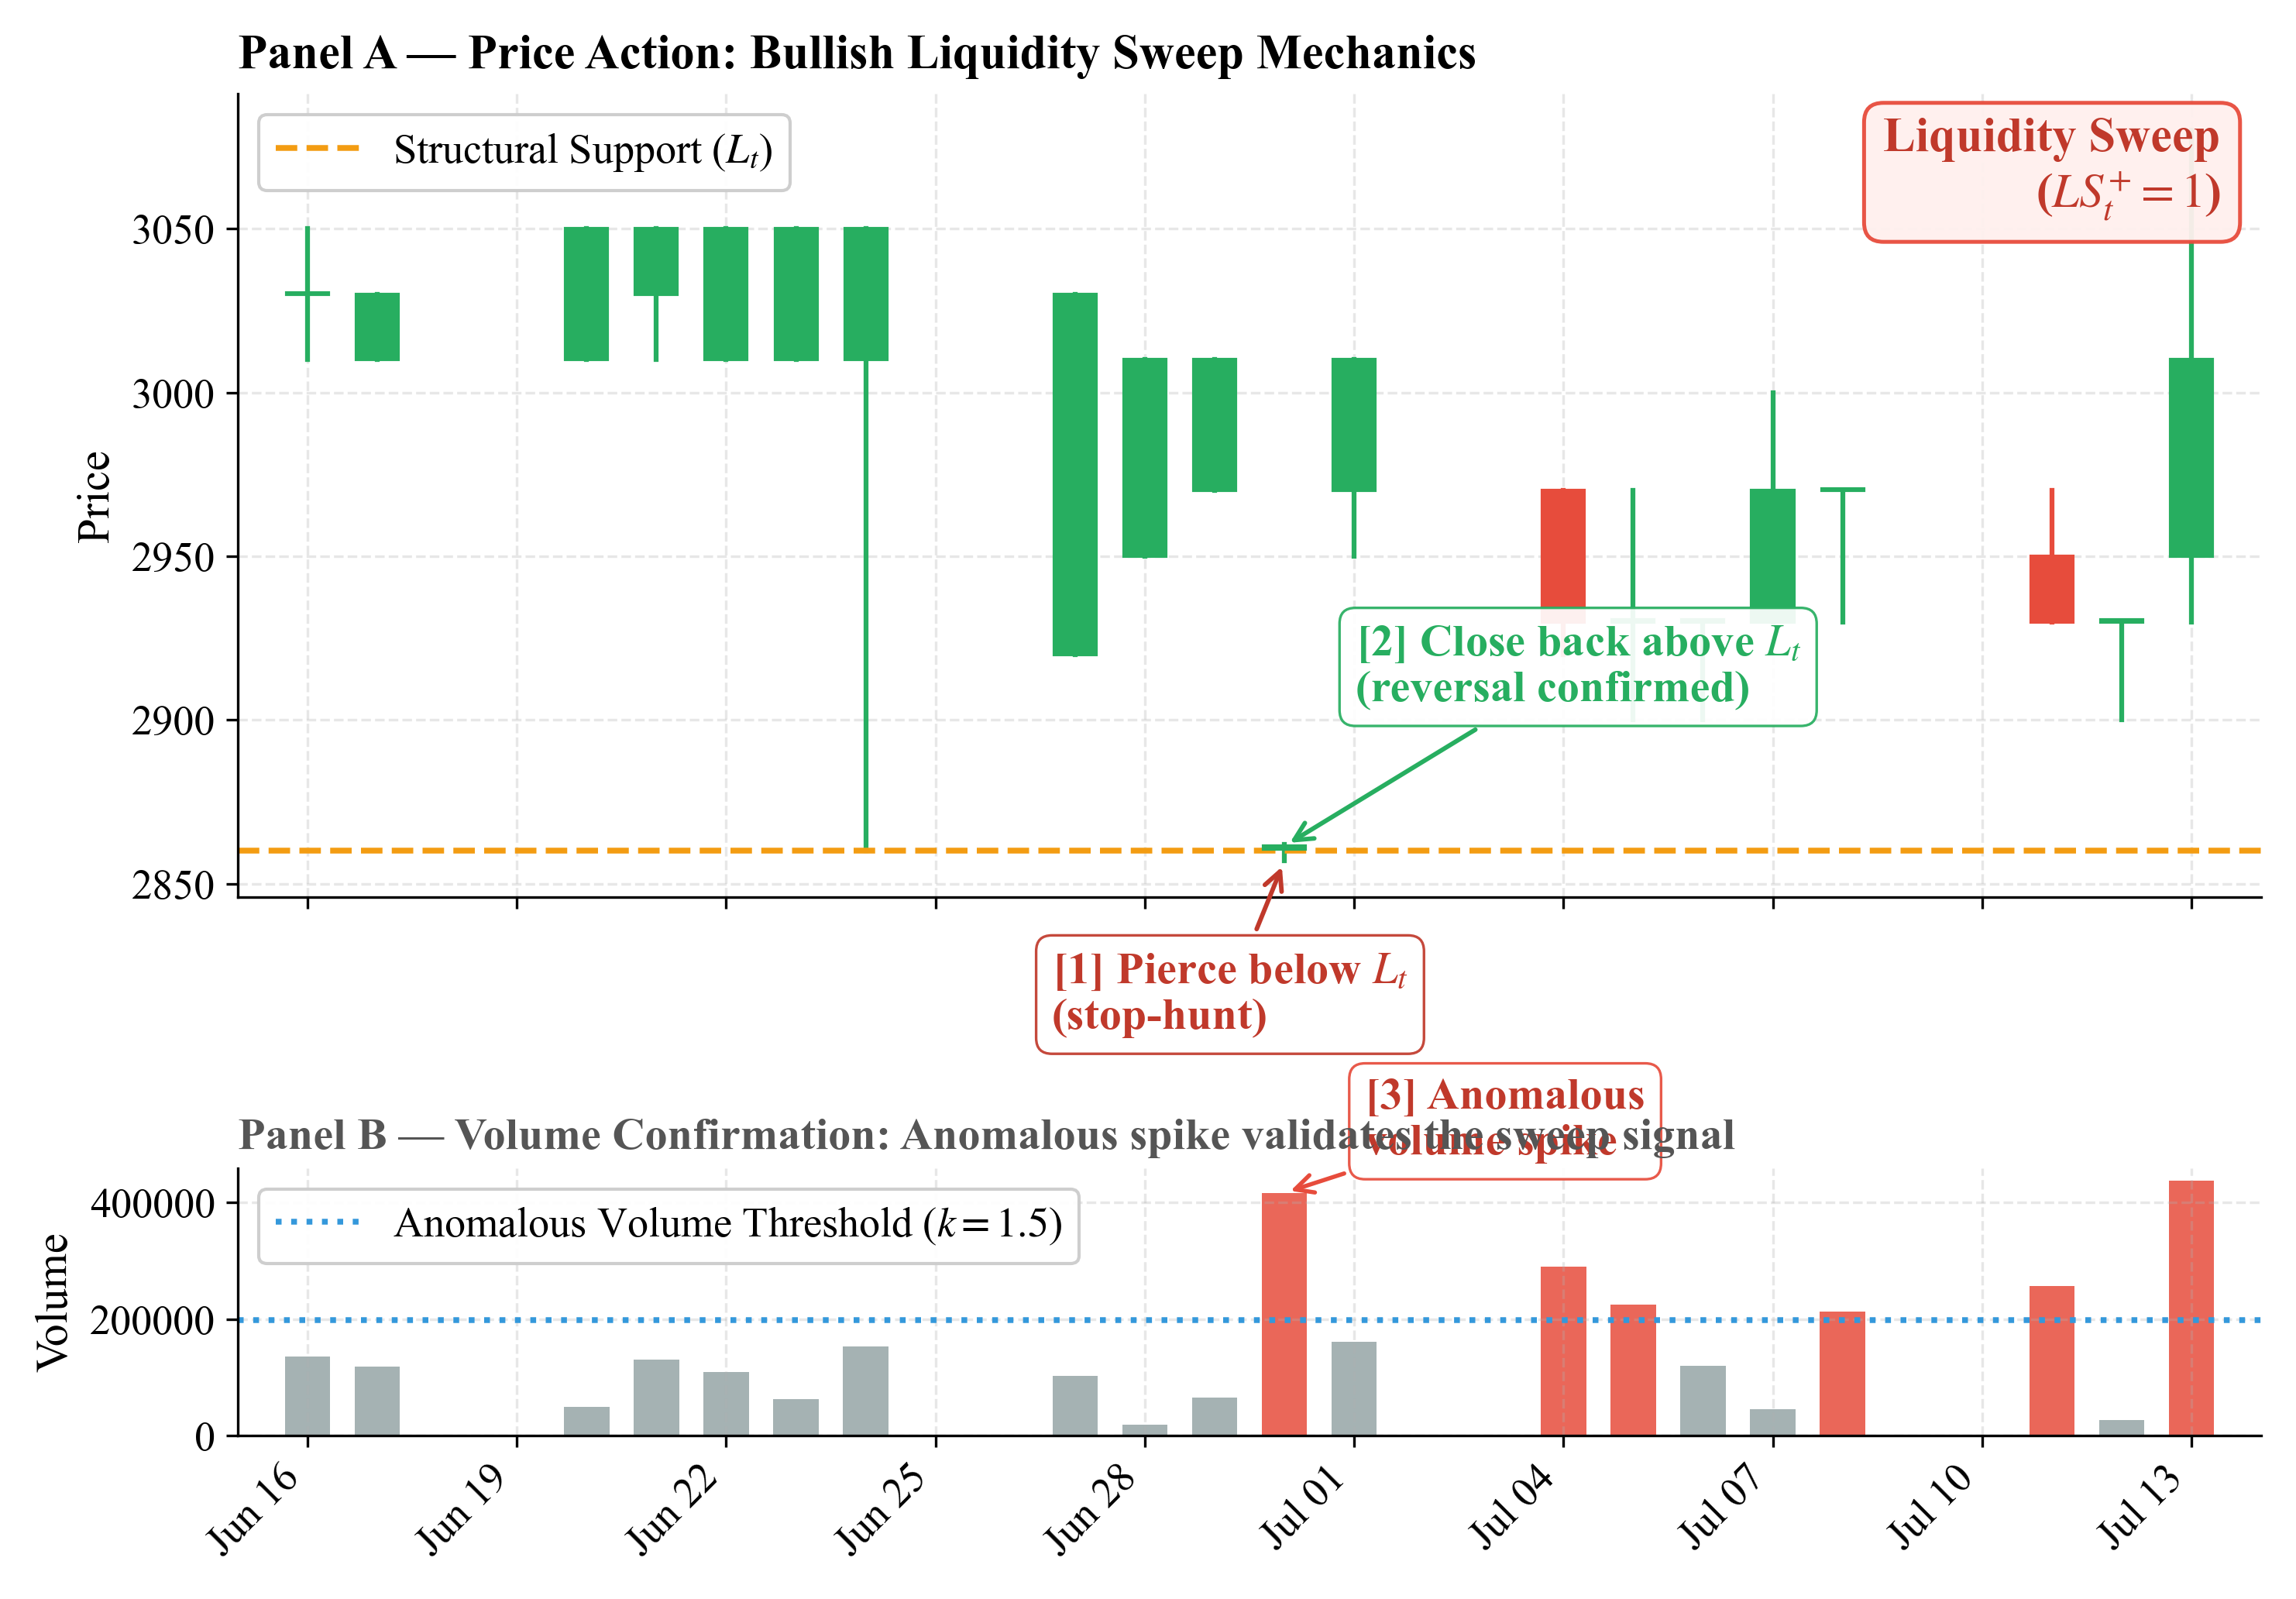
\includegraphics[width=\linewidth]{images/liquidity_sweep_anatomy.png}
    \caption{Anatomy of an Institutional Liquidity Sweep. Step [1]: price temporarily pierces the structural support $L_t$ (the 20-day swing low), triggering clustered retail stop-loss orders. Step [2]: price immediately reverses and closes back above $L_t$, confirming institutional absorption. Step [3]: the piercing candle is accompanied by an anomalous volume spike exceeding the $k{=}1.5$ threshold, providing the volume-confirmation criterion for $LS_t^{+}{=}1$.}
    \label{fig:sweep_anatomy}
    \end{figure}

    \begin{figure}[htbp]
    \centering
    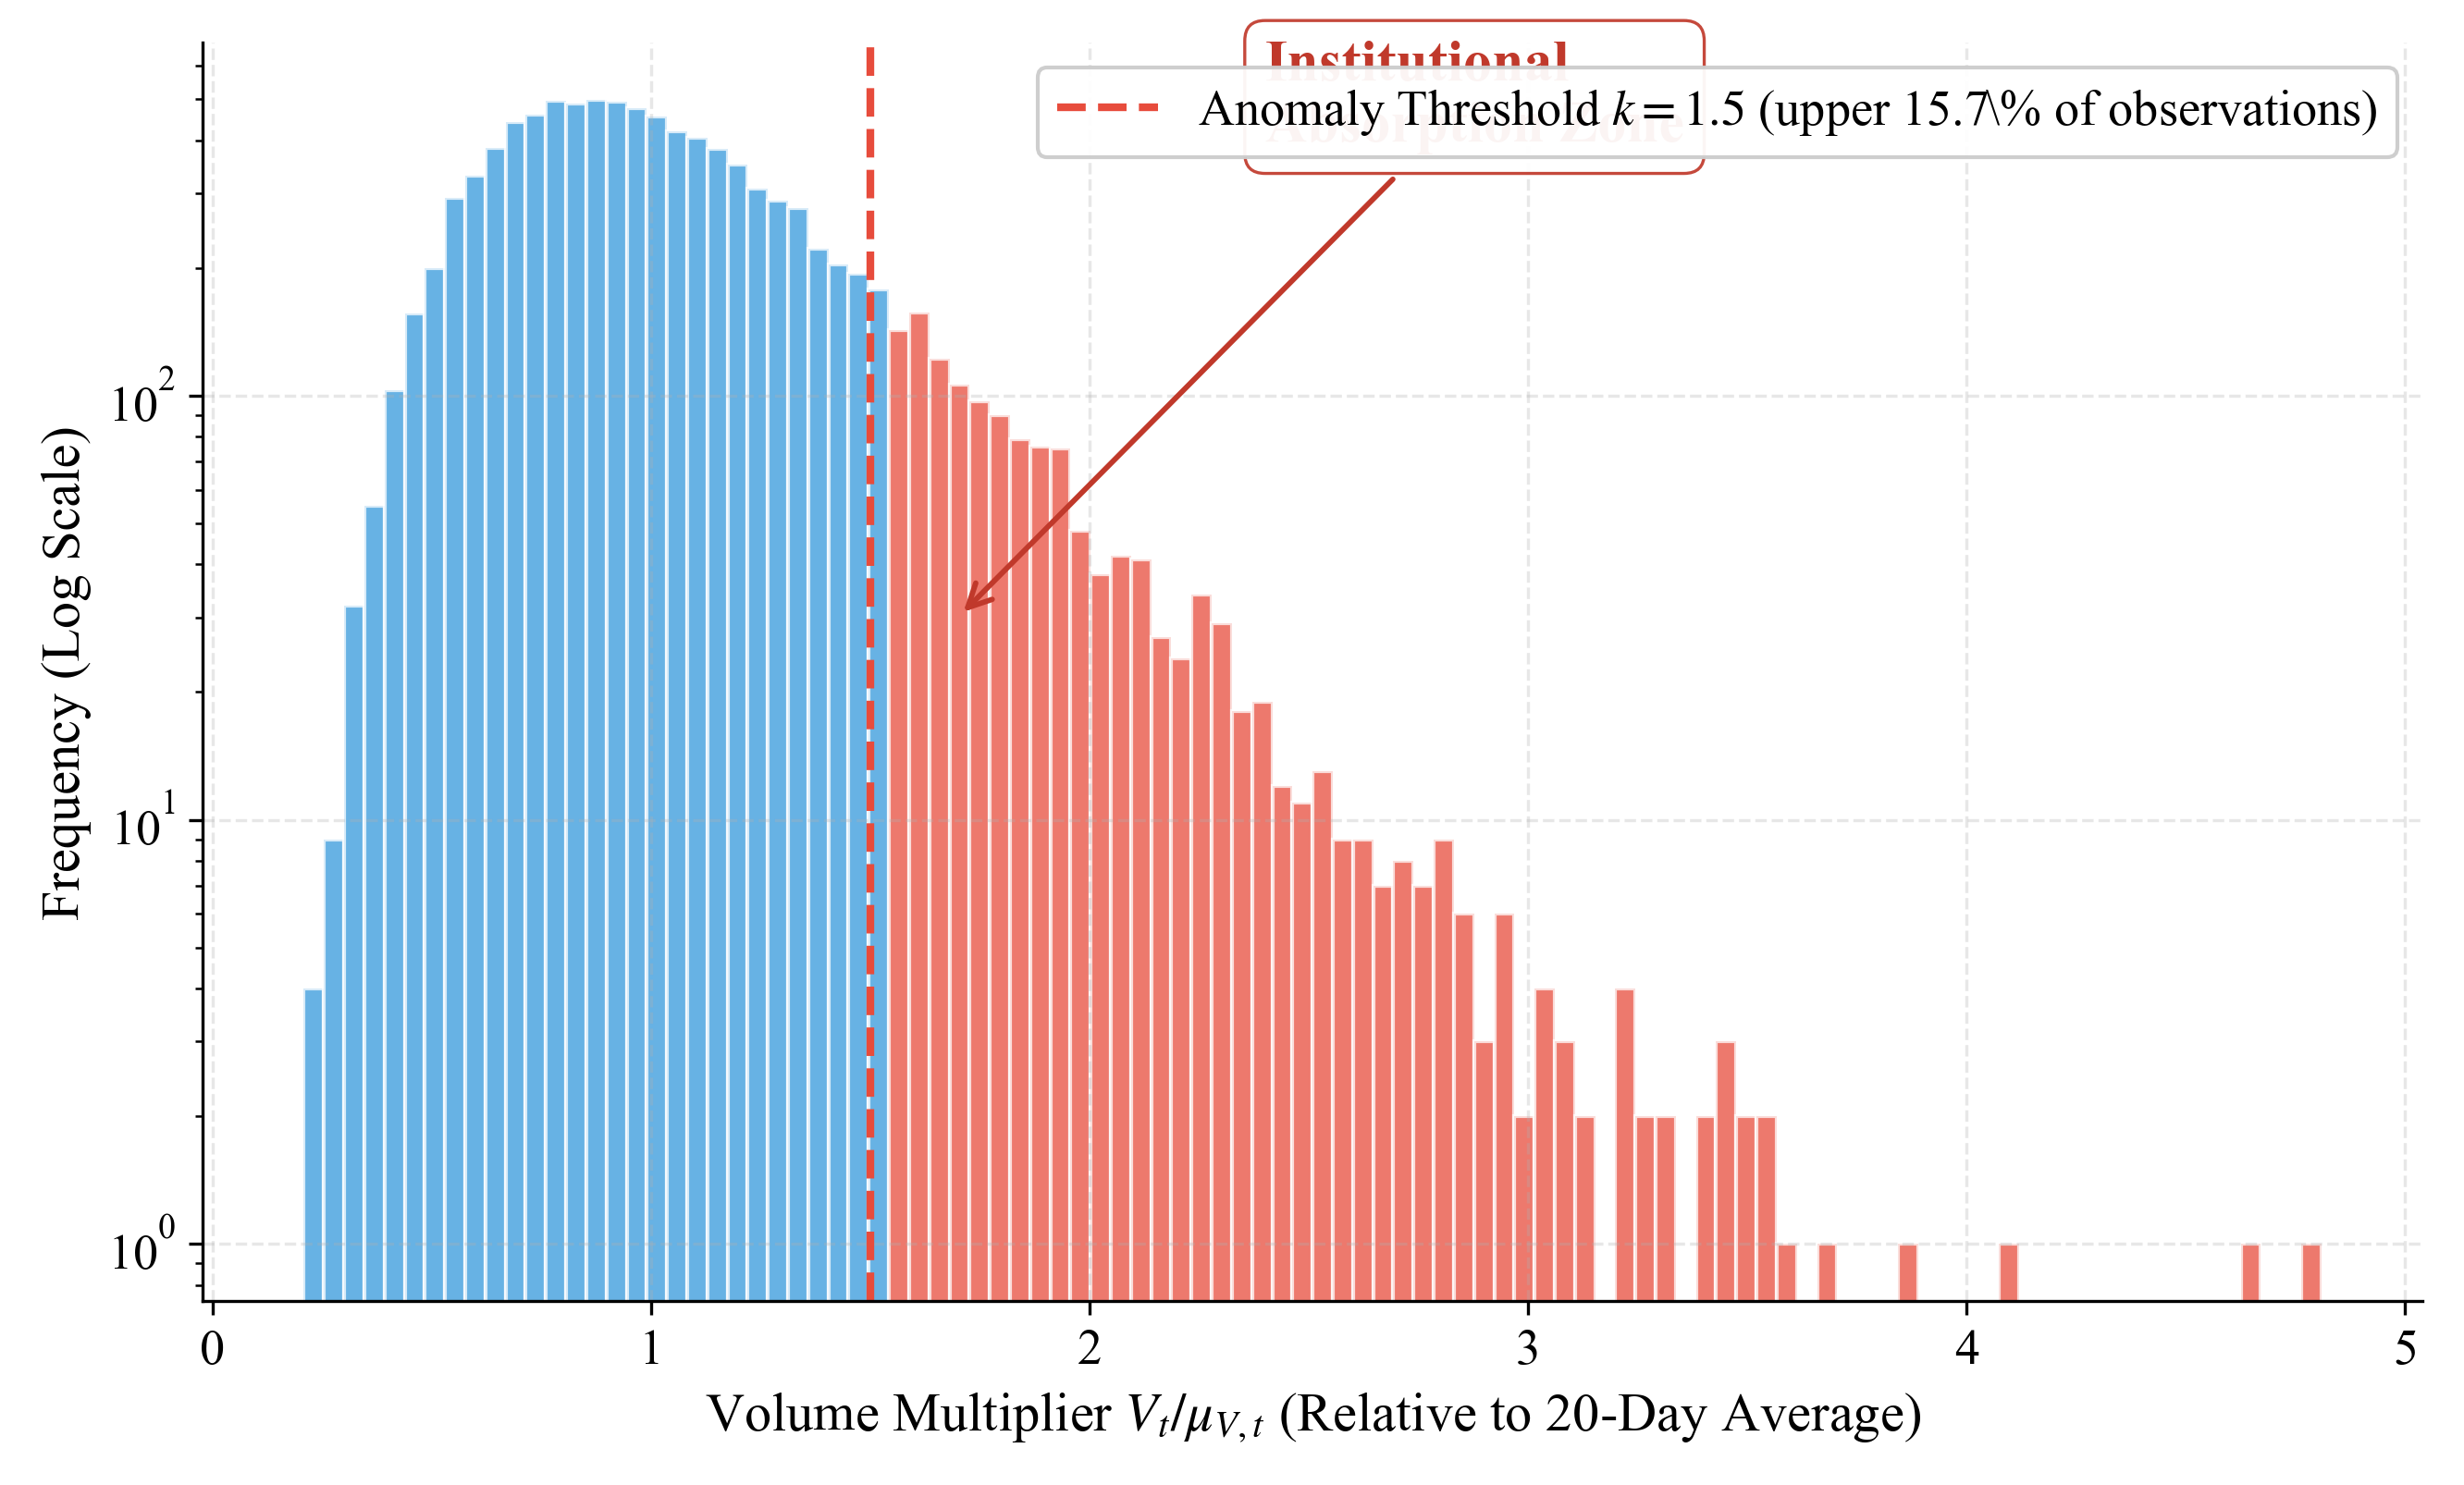
\includegraphics[width=0.95\linewidth]{images/volume_histogram.png}
    \caption{Empirical distribution of the relative volume multiplier $V_t / \mu_{V,t}$ across the 10-year VN30 dataset, fitted to a log-normal model. Blue bars represent the bulk of normal trading activity; red bars denote observations exceeding the institutional-intervention threshold $k{=}1.5$. The rarity of these upper-tail events (${\approx}20\%$ of trading days) motivates their use as a discriminative feature for flagging Liquidity Sweeps.}
    \label{fig:volume_hist}
    \end{figure}

    \subsection{Deep Predictive Architectures}
    The resultant pure price-action SMC dataset serves as the training corpus designed to predict post-shakeout price trajectories. We benchmark four fundamentally different architectures:
    \begin{itemize}
        \item \textbf{LightGBM:} An advanced tree-based gradient boosting framework functioning as our non-temporal baseline.
        \item \textbf{LSTM:} A classical recurrent neural network evaluating longitudinal dependencies in market data.
        \item \textbf{iTransformer:} An inverted Transformer topology that separately embeds the entire historical series of individual features.
        \item \textbf{PatchTST:} A sophisticated Transformer implementation that segments temporal series into overlapping local patches to preserve localized sub-sequence patterns.
    \end{itemize}

    \begin{figure}[htbp]
    \centering
    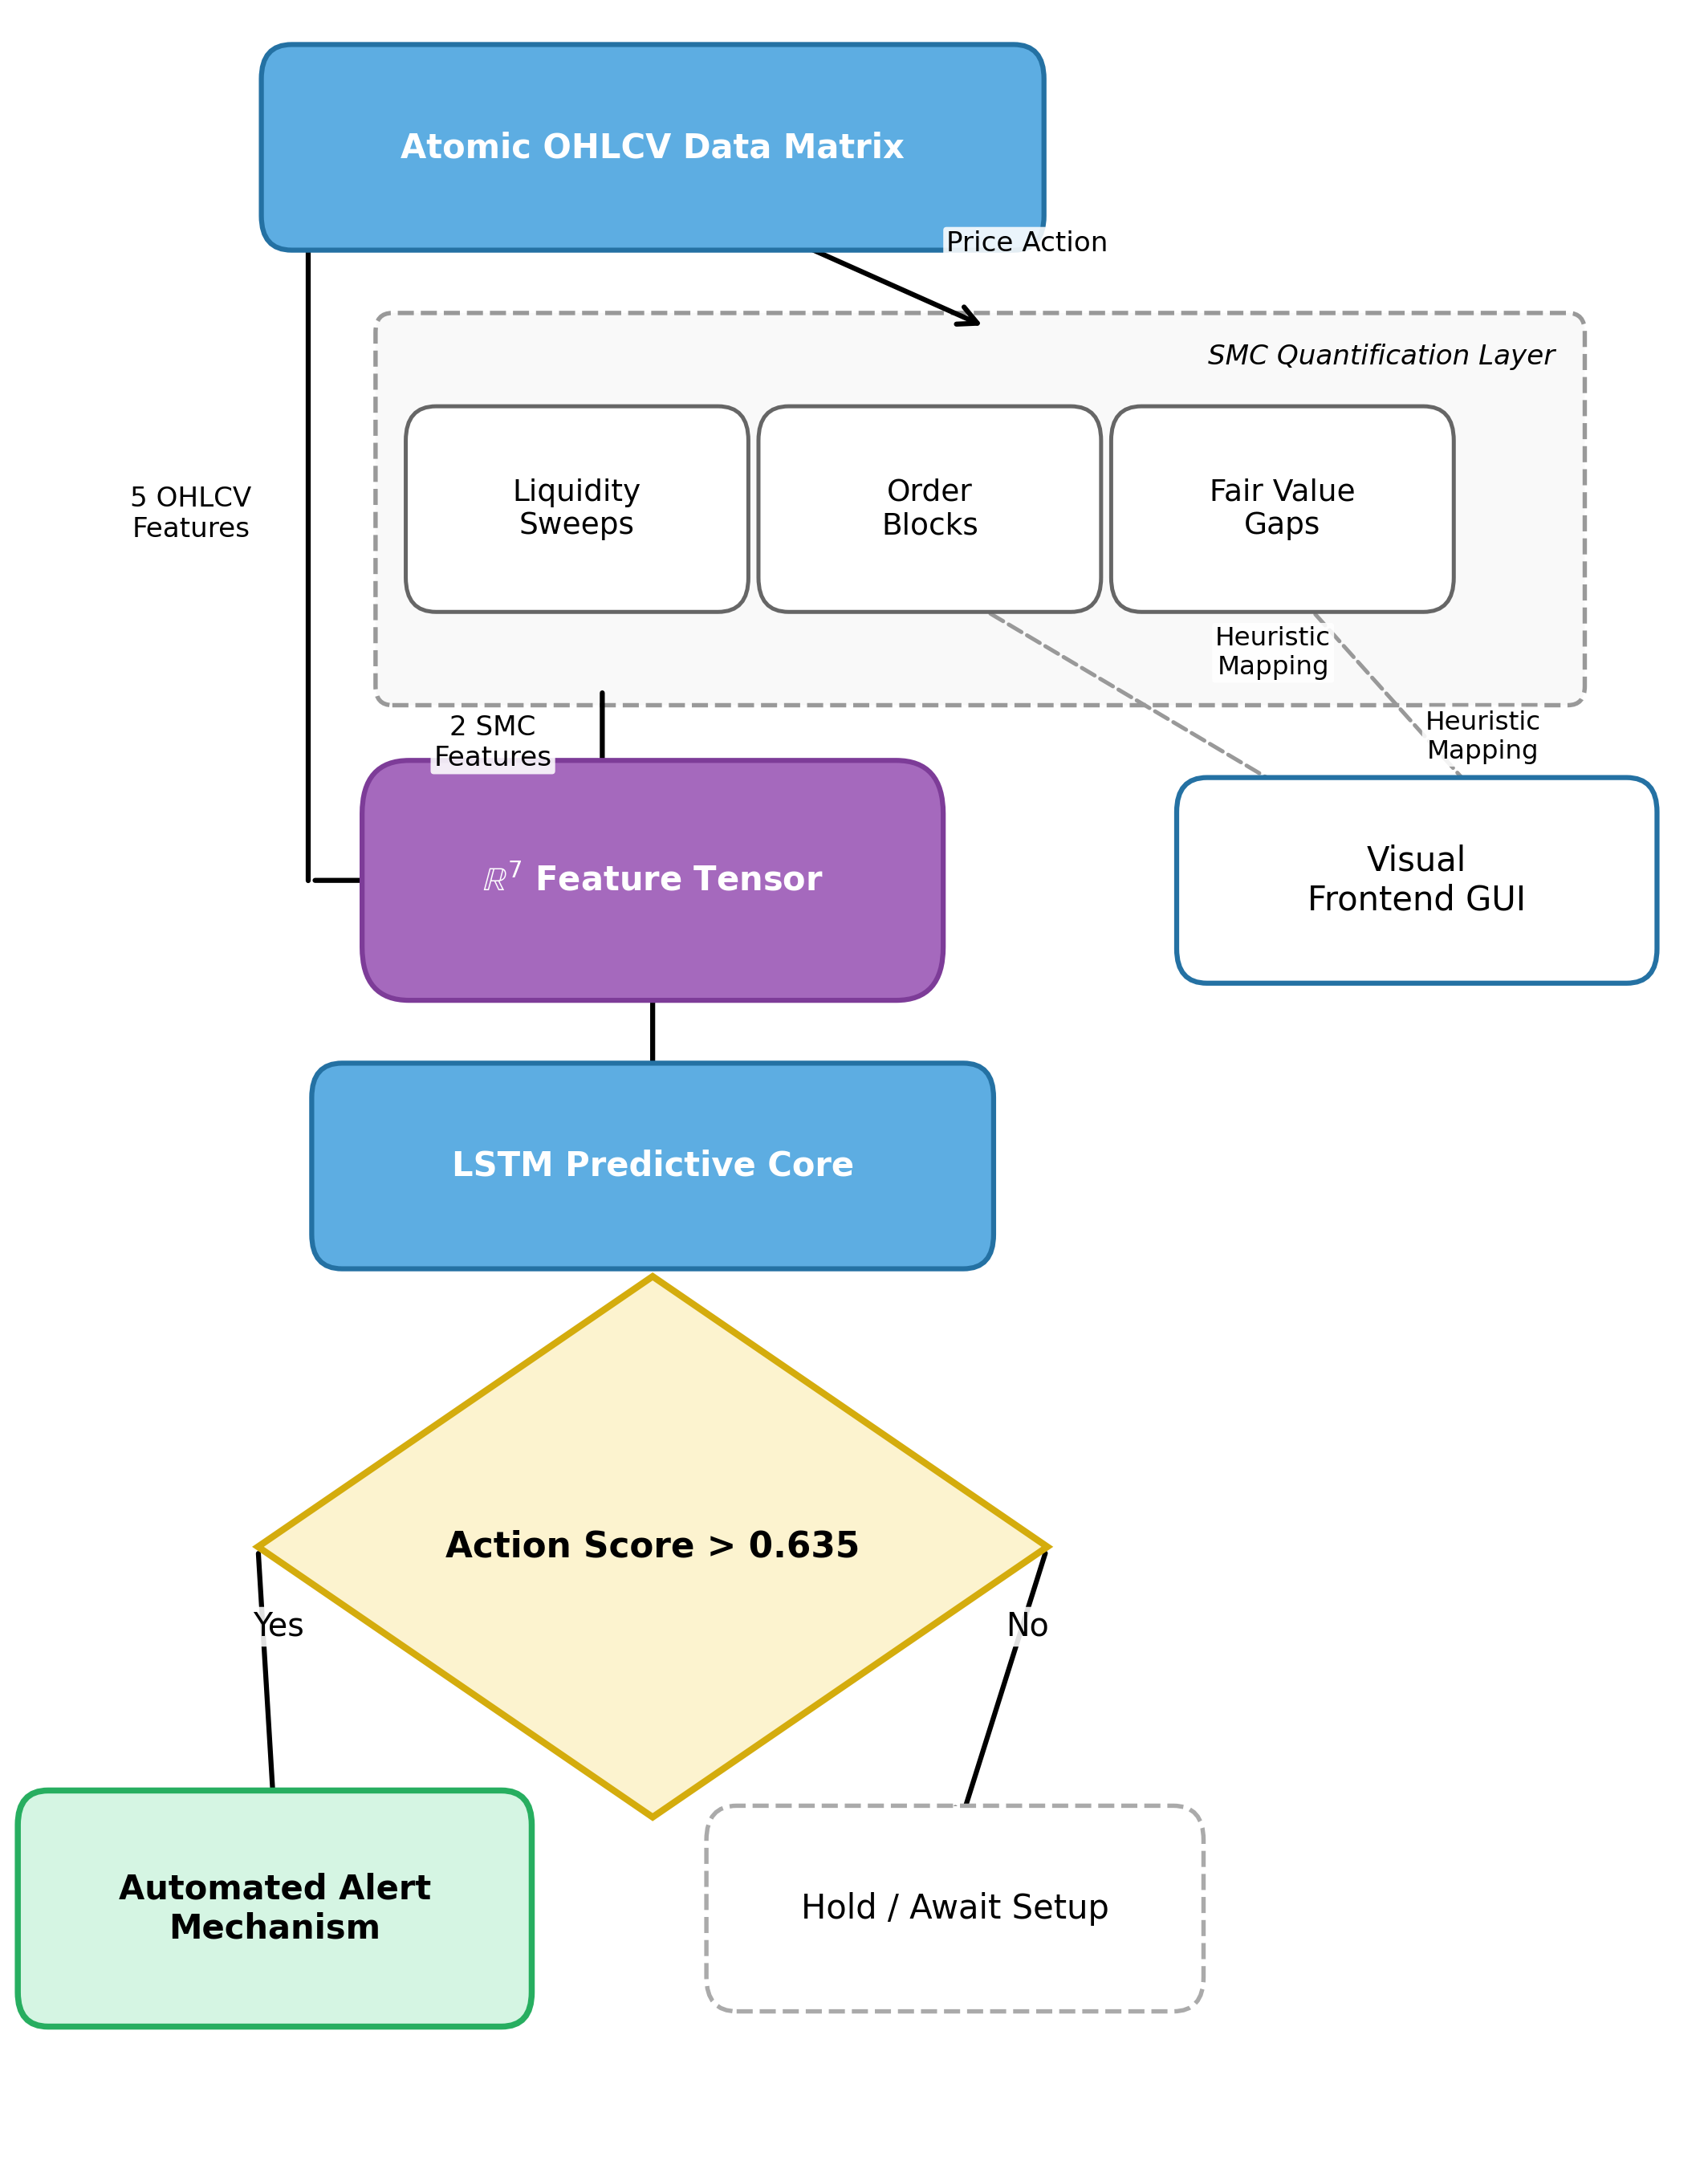
\includegraphics[width=\linewidth]{images/system_architecture.png}
    \caption{The Green Dragon System Architecture: end-to-end pipeline from raw OHLCV ingestion through SMC quantification, RobustScaler preprocessing, and the four benchmarked predictive engines (LightGBM, LSTM, iTransformer, PatchTST) to the transaction-cost-adjusted Action Score output.}
    \label{fig:architecture}
    \end{figure}

    \subsection{Data Preprocessing and Robust Scaling}
    During the dataset construction, traditional lagging indicators (such as RSI and MACD) were explicitly excluded to test the true efficacy of SMC features. This empirical framework relies on the careful handling of 10 years of VN30 OHLCV data. The final input feature matrix comprises \textbf{7 dimensions}: five price-action channels derived from OHLCV (Open, High, Low, Close returns via \texttt{pct\_change()}, and Volume via \texttt{log1p().diff()}), augmented with two deterministic SMC indicators---the composite sweep indicator ($LS_t \in \{-1, 0, 1\}$) and its continuous strength scalar ($LS_{\text{strength},t}$).

    A critical preprocessing phase involves the treatment of extreme volume spikes. Clipping infinite values to zero inadvertently blinds the model to true institutional footprints. Instead, we implement a \texttt{RobustScaler} (using Interquartile Range) to standardize the five OHLCV channels without destroying extreme accumulation outliers, while the two SMC features are passed through unchanged. To definitively preclude look-ahead bias, the \texttt{RobustScaler} is fitted \emph{exclusively} on the training partition (64\% of the chronological dataset) and subsequently applied as a frozen transform to the validation and test partitions \cite{prado2018advances}.

    \section{Proof-of-Concept: Visual Explainability (XAI) Architecture}
    The central contribution of this section is not application deployment, but rather demonstrating how the LSTM's latent predictions can be deterministically mapped back onto observable market structures to achieve interpretability---directly addressing the ``black-box'' critique levelled at deep learning in finance \cite{arrieta2020explainable}.

    LSTM is implemented as the core algorithmic engine within the pipeline illustrated in Figure~\ref{fig:architecture}. The engine processes data through the SMC quantification layer, building a \textbf{7-dimensional feature tensor} $\mathbf{x}_t \in \mathbb{R}^{7}$ per trading day: $(\Delta_\text{open}, \Delta_\text{high}, \Delta_\text{low}, \Delta_\text{close}, \Delta_\text{volume}, LS_t, LS_{\text{strength},t})$. A sliding window of $T=20$ consecutive trading days forms each model input $(\mathbf{x}_{t-19}, \ldots, \mathbf{x}_t) \in \mathbb{R}^{20 \times 7}$, enabling the LSTM to decode temporal institutional footprints, ultimately outputting an \textit{Action Score} $\hat{y}_t \in [0, 1]$.

    Rather than relying on probability calibration (e.g., Platt Scaling), which enforces a static 0.5 threshold optimized for symmetric log-loss and thus ignores asymmetric transaction costs \cite{almgren2001optimal}, our system employs a Bayesian Optimization framework (Optuna \cite{akiba2019optuna}) to discover a dynamically tuned threshold ($\hat{y} = 0.635$) that directly maximizes the simulated out-of-sample Sharpe Ratio. It is important to acknowledge a limitation of this approach: a threshold optimized on the validation partition carries an inherent risk of cross-regime threshold overfitting. The threshold may not generalize optimally to unseen market conditions beyond the VN30 test window, and its robustness across different emerging market indices remains unverified.

    The XAI layer renders explicit structural markers (BOS, CHoCH) and localized Risk/Reward parameters (T+2.5 adjusted Stop-Loss and Take-Profit zones) directly on the graphical interface, enabling traders to visually verify the confluence between the algorithmic Action Score and the underlying SMC structures. This addresses the interpretability gap identified in \cite{mdpi2024review} without requiring post-hoc explanation methods such as SHAP or LIME, since the features themselves are grounded in observable price structure.

    To eliminate manual tape reading, Action Scores are evaluated against the tuned threshold to dispatch automated alerts. An integrated generative AI chatbot provides natural language explanations of triggered signals. Future iterations will formally integrate Order Blocks and CHoCH into the quantitative tensor, enabling richer structural explainability.

    \begin{figure}[htbp]
    \centering
    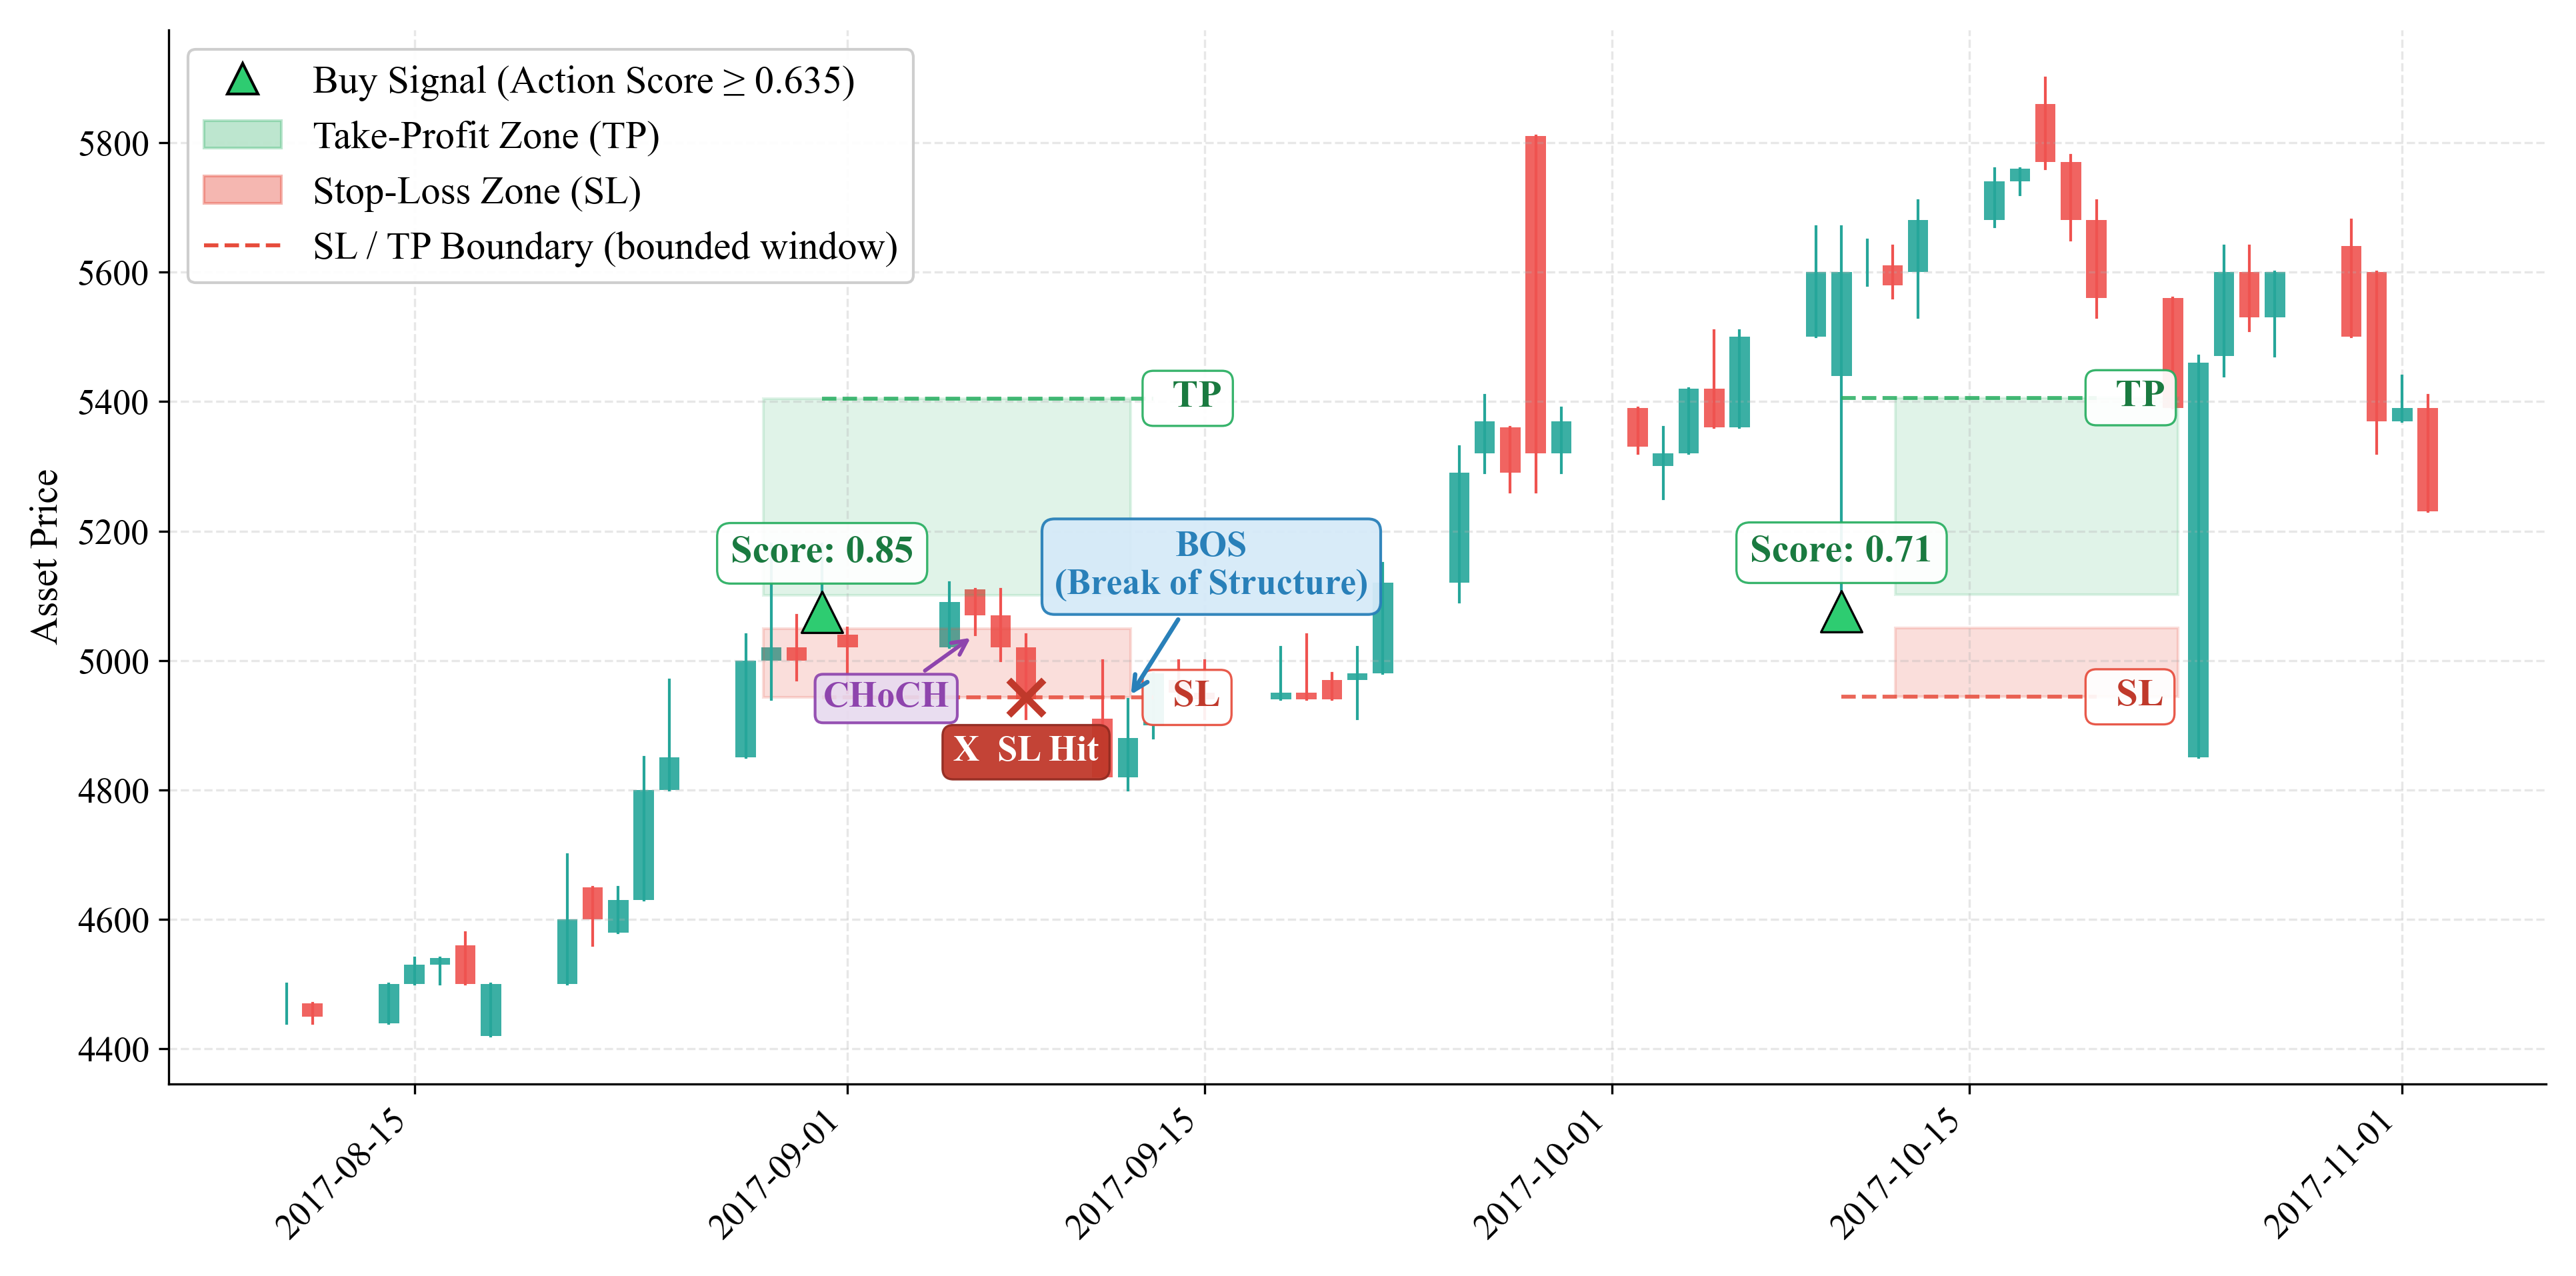
\includegraphics[width=\textwidth]{images/signal_overlay.png}
    \caption{Green Dragon XAI Execution Overlay: price action annotated with LSTM buy signals (green triangles, Action Score $\hat{y}{>}0.635$) and two key SMC structural markers---Break of Structure (BOS, blue: price breaks a prior swing high, confirming bullish intent) and Change of Character (CHoCH, purple: momentum reversal after a Liquidity Sweep). Each triggered signal is accompanied by dynamically computed Stop-Loss (SL, red zone) and Take-Profit (TP, green zone) levels, rendering the LSTM's latent predictions directly interpretable on observable price structure.}
    \label{fig:signal_overlay}
    \end{figure}

    \section{Experiments and Results}

    \subsection{Evaluation Metrics \& Optuna Framework}
    To ascertain the practical financial viability of the quantitative models on the pure price-action SMC dataset, we simulate algorithmic portfolio returns to derive risk-adjusted metrics, specifically the Annualized Sharpe Ratio and Maximum Drawdown (MDD). The framework stringently prevents temporal data leakage by utilizing an expanding 252-day window to calculate a trailing 20-day historical volatility, reliably routing daily features into 3 continuous partitions: Regime 1 (Stable), Regime 2 (Normal), and Regime 3 (Extreme). 

    \begin{figure}[htbp]
    \centering
    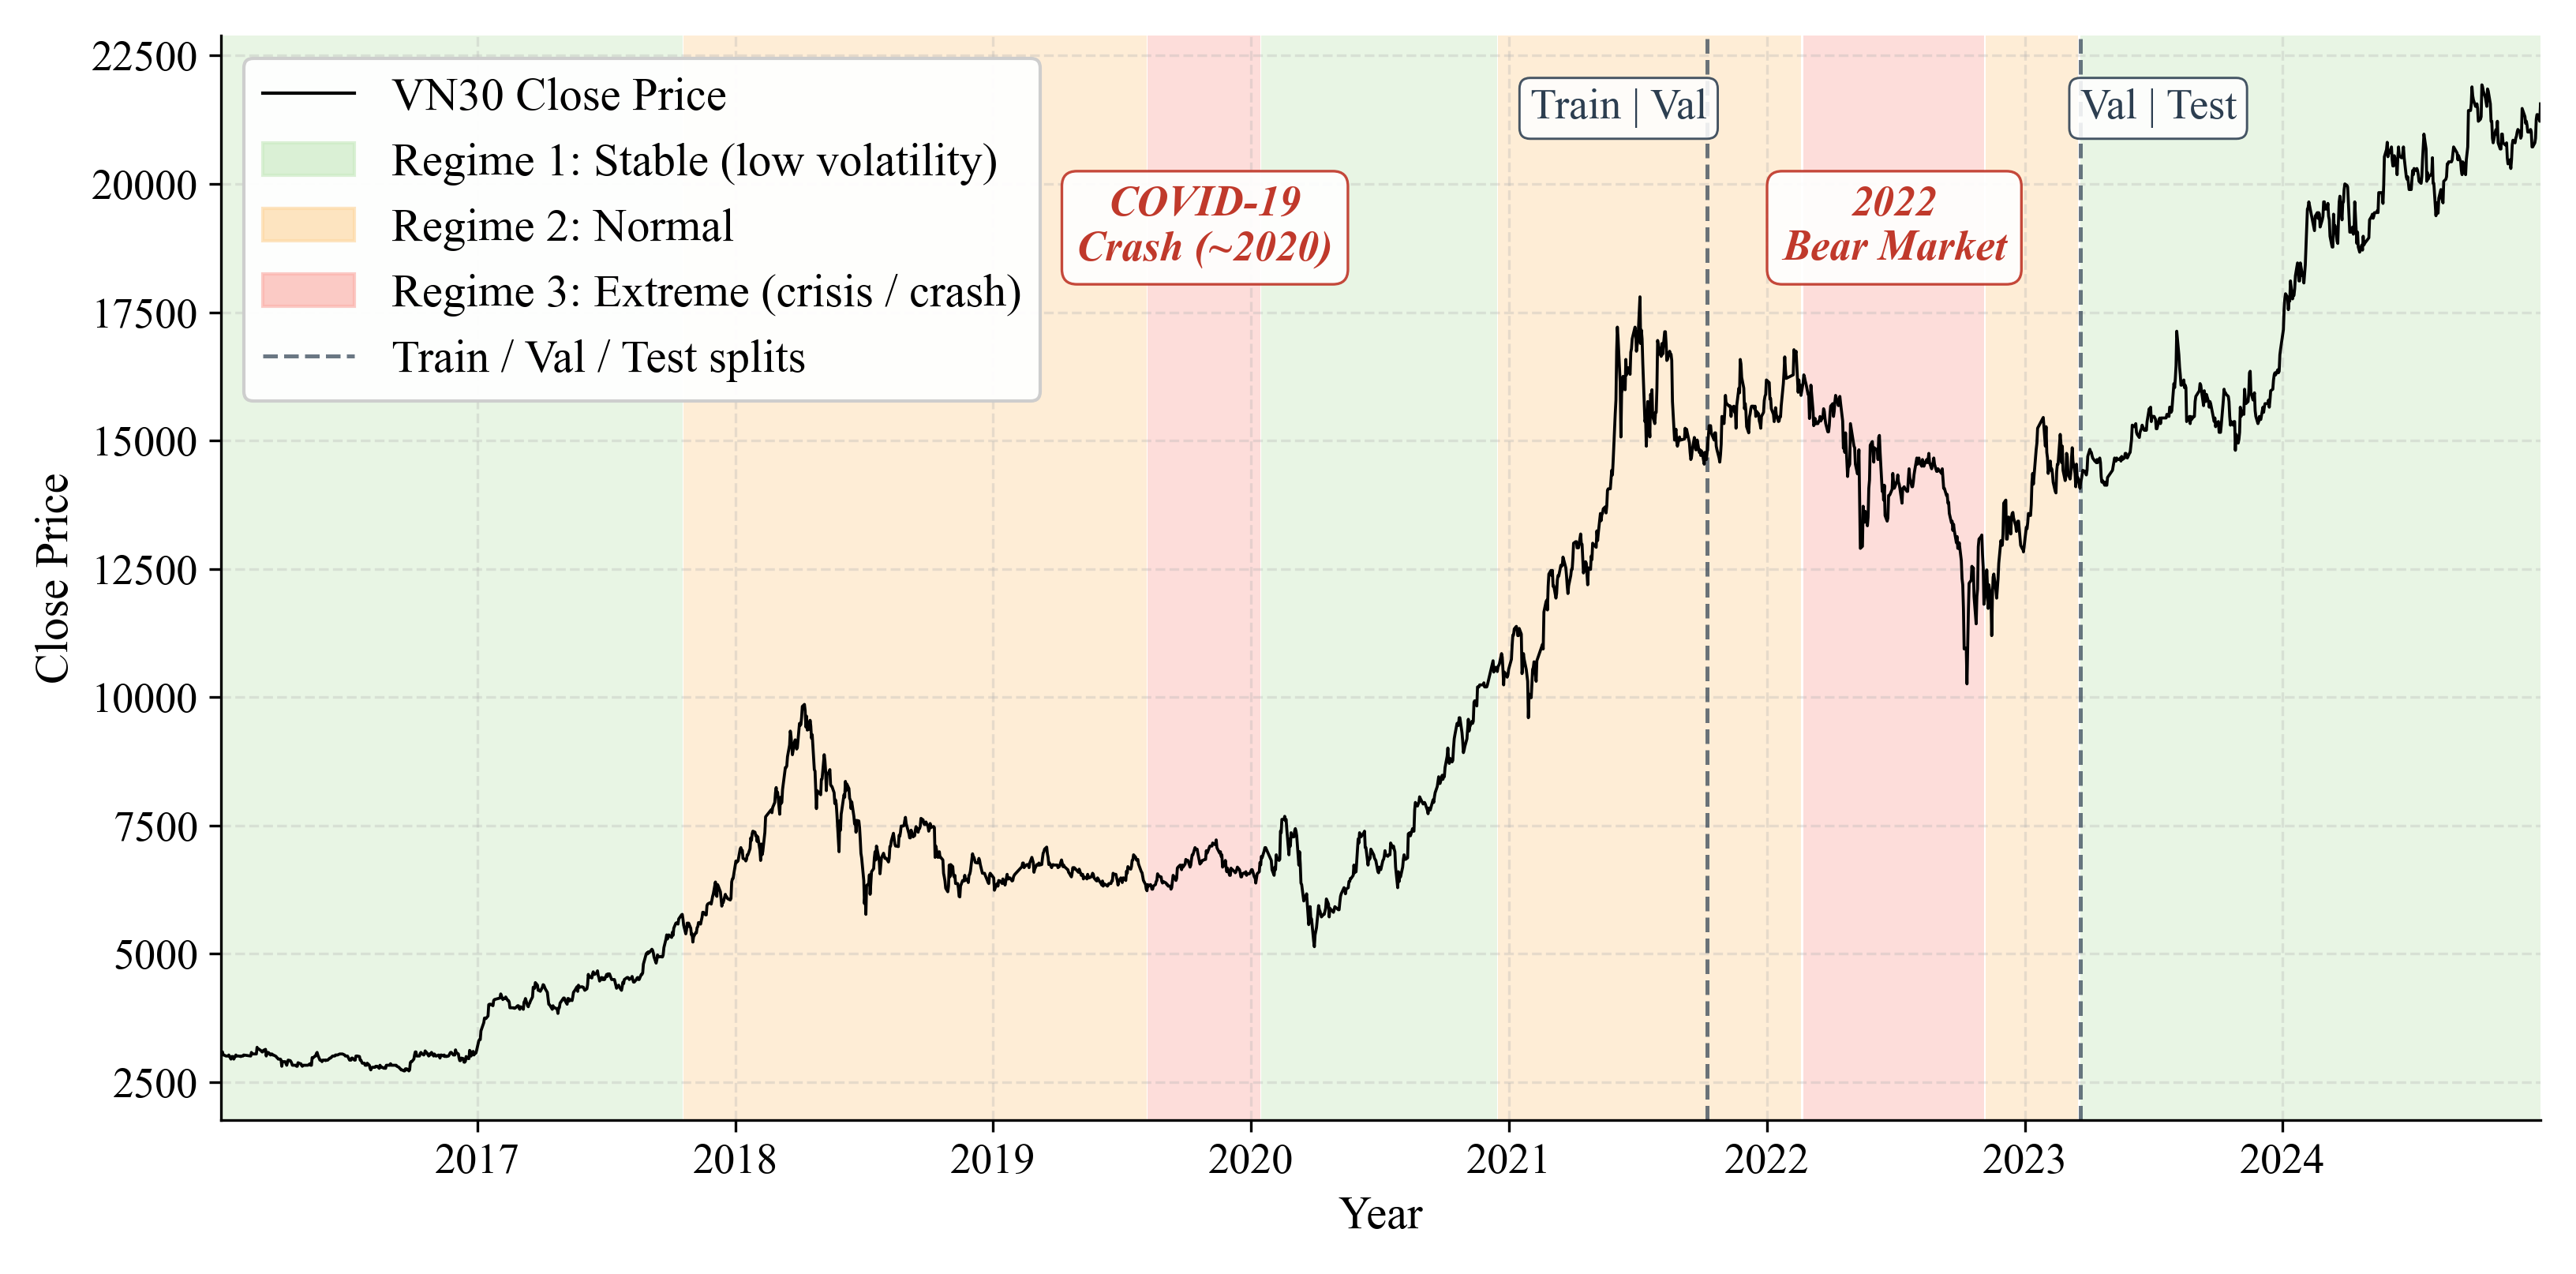
\includegraphics[width=\linewidth]{images/market_regimes.png}
    \caption{Market Regime Switching Overlay (2014--2024): volatility-based chronological segmentation of the VN30 index into three regimes---Regime~1 (Stable, green), Regime~2 (Normal, orange), and Regime~3 (Extreme, red). Key crisis events (COVID-19 crash, 2022 Bear Market) are annotated within their respective Extreme windows. Dashed vertical lines indicate the 64/16/20 chronological Train/Validation/Test split boundaries.}
    \label{fig:market_regimes}
    \end{figure}

    A continuous 3-way chronological split (64\% Train, 16\% Val, 20\% Test) is evaluated in connection with an Optuna optimization search isolating the ideal learning hyperparameters and optimal Long-Only predictive Action Score bounds required to surpass $0.25\%$ transaction decay.

    \begin{figure}[htbp]
    \centering
    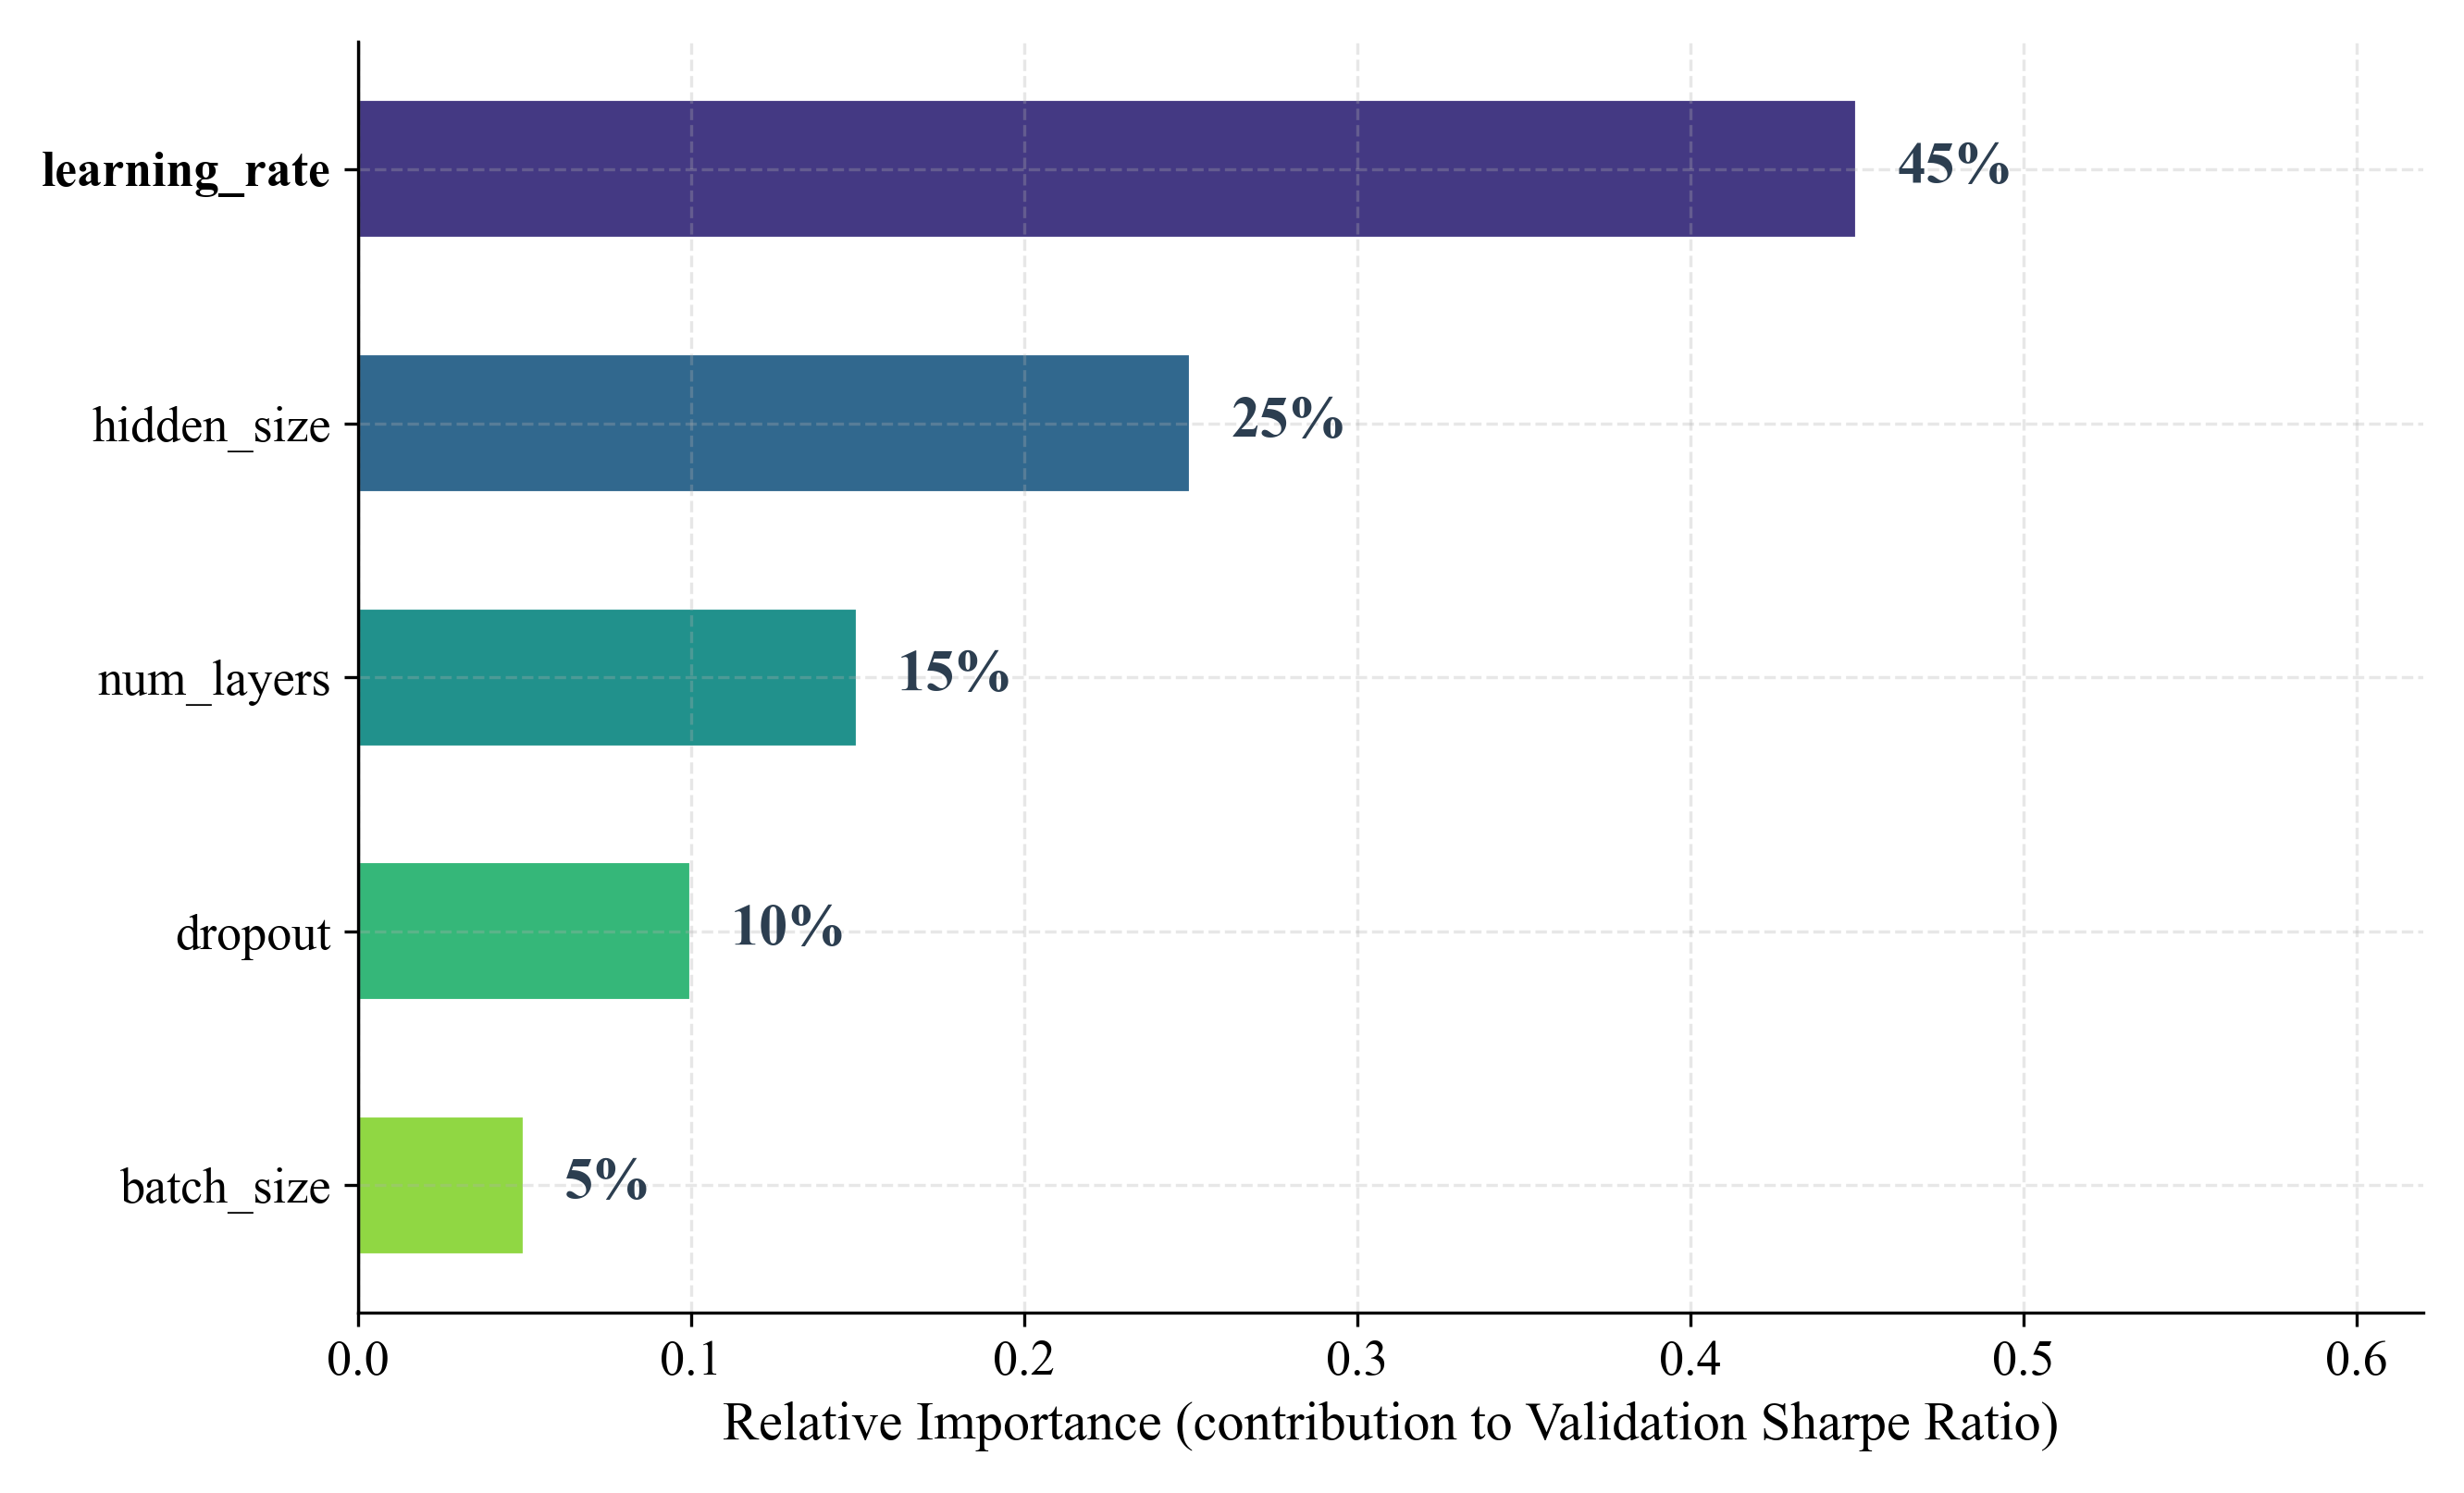
\includegraphics[width=0.85\linewidth]{images/optuna_importance.png}
    \caption{Optuna hyperparameter importance scores quantifying each parameter's relative contribution to the LSTM validation Sharpe Ratio. \texttt{learning\_rate} dominates (45\%), followed by \texttt{hidden\_size} (25\%), confirming that gradient-step magnitude and model capacity are the primary levers for this dataset scale.}
    \label{fig:optuna_importance}
    \end{figure}

    \begin{figure}[htbp]
    \centering
    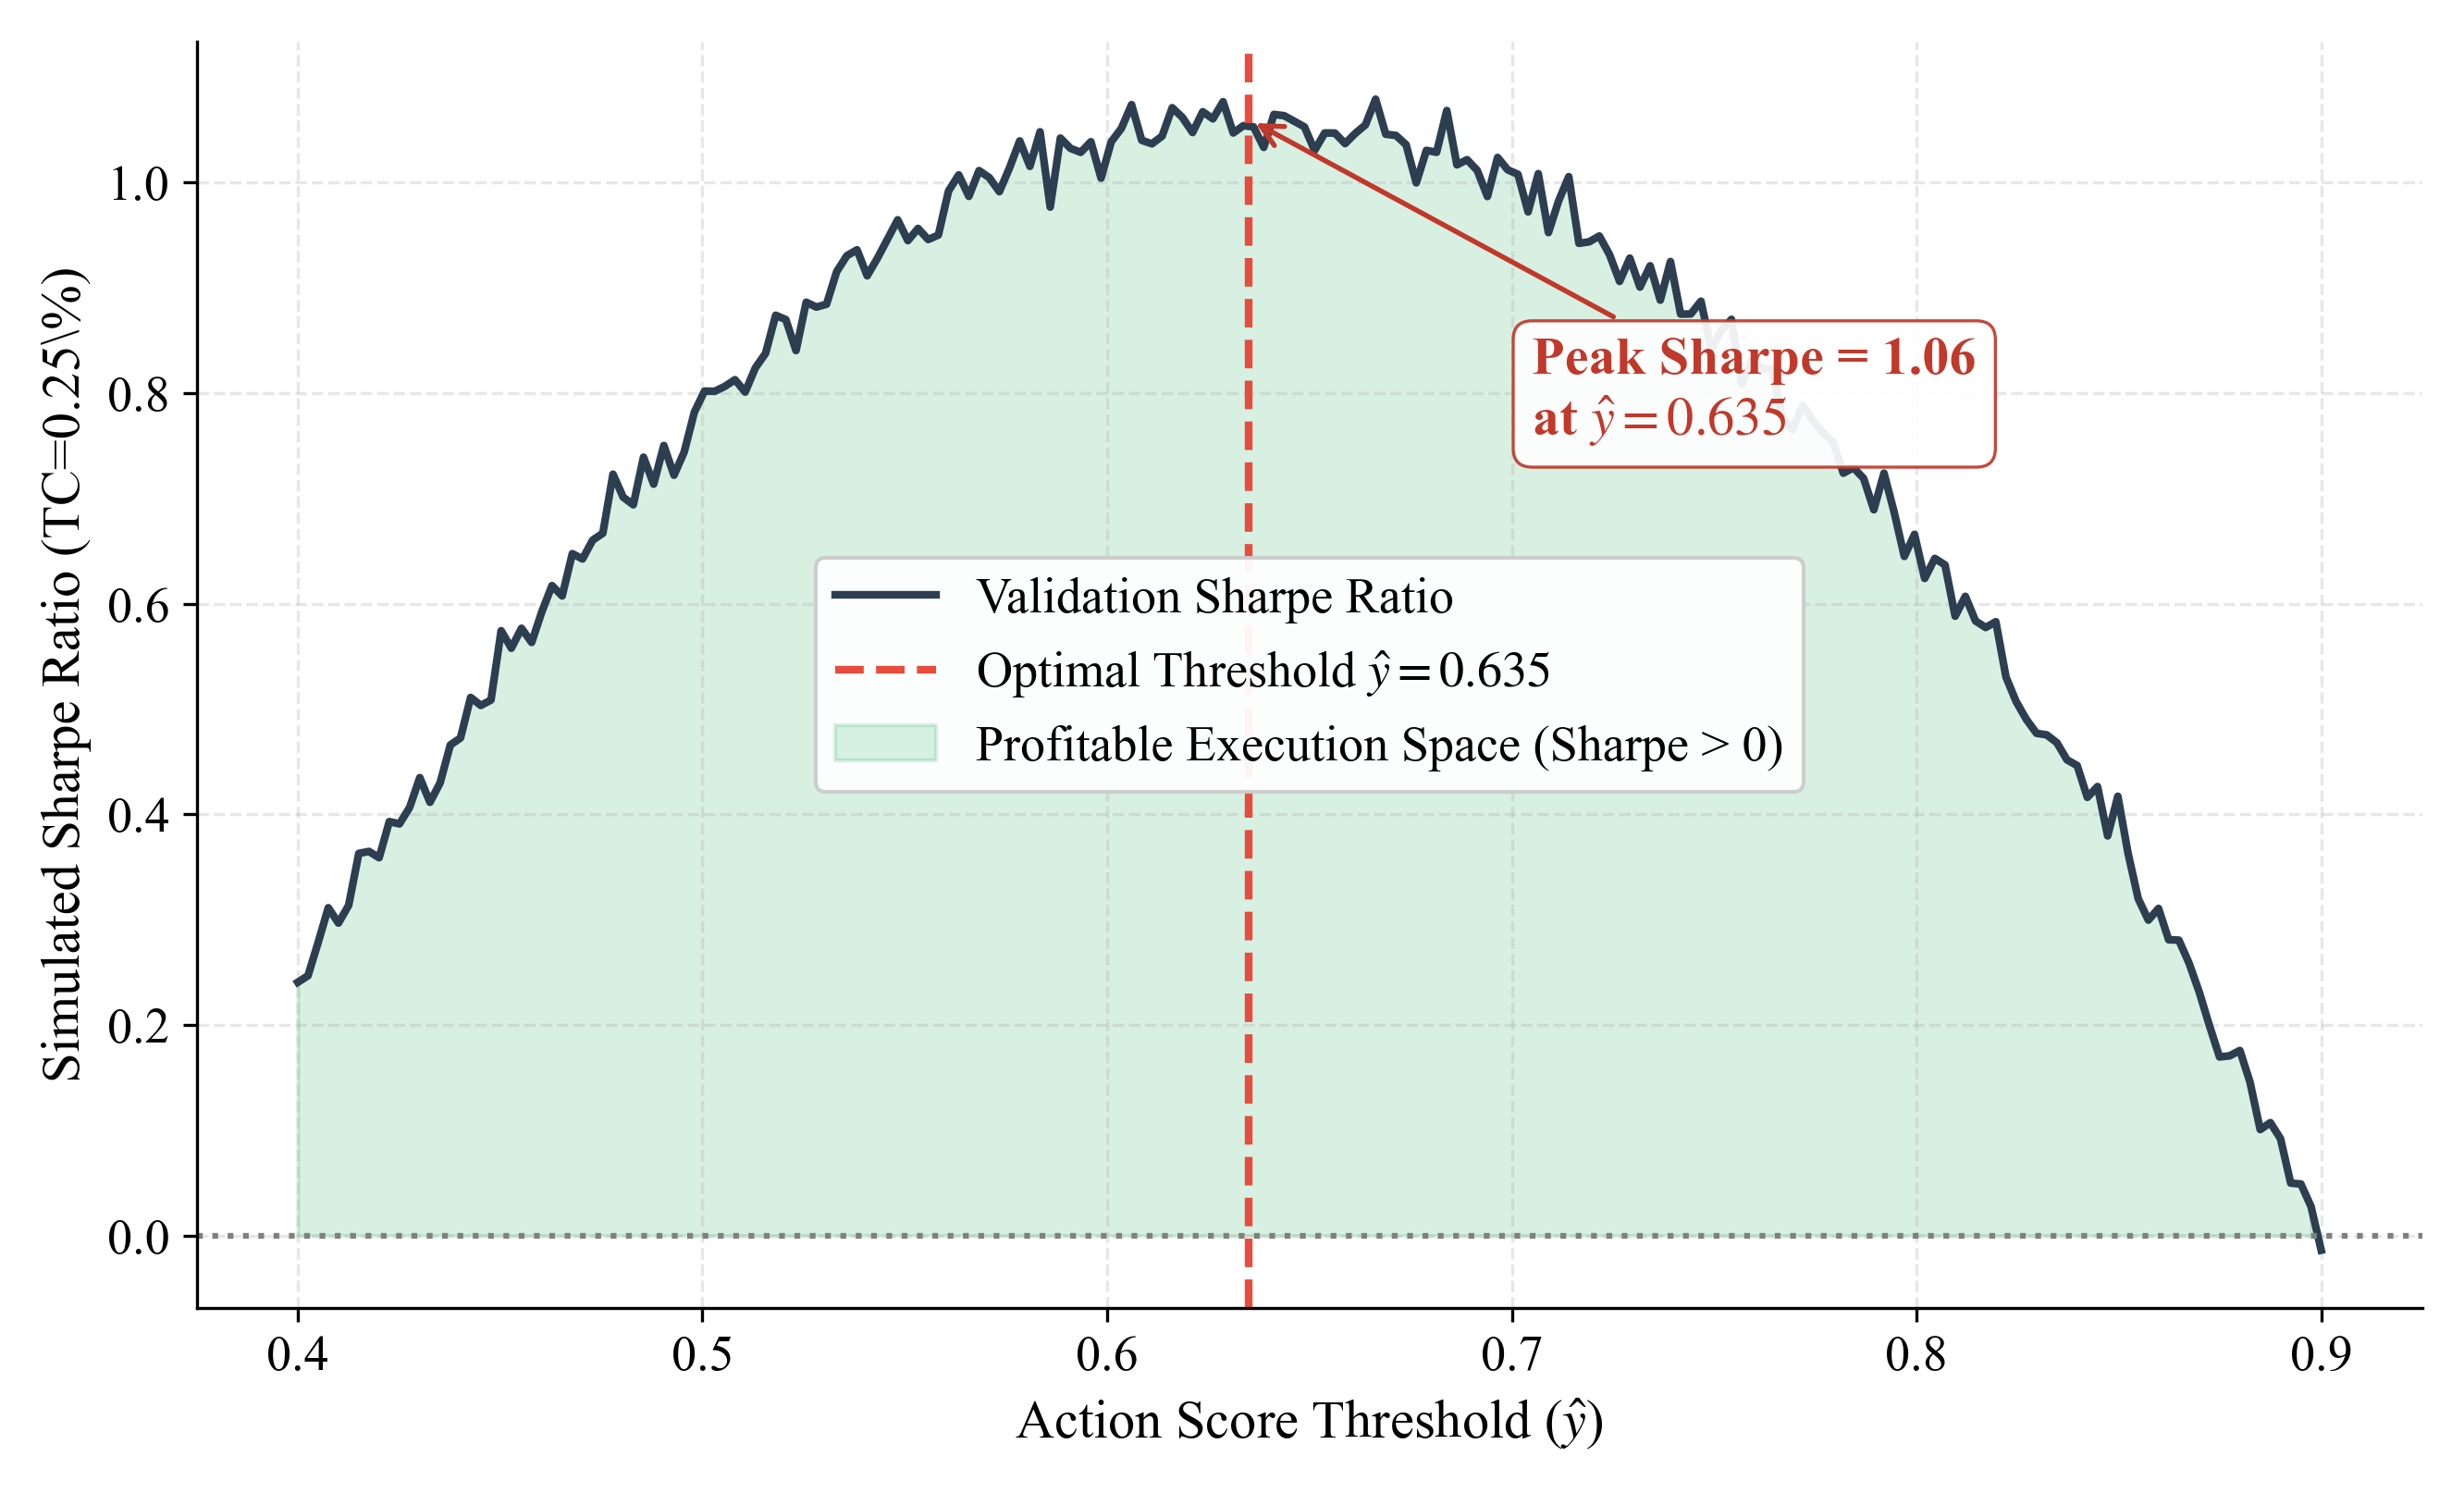
\includegraphics[width=\linewidth]{images/dynamic_threshold.png}
    \caption{Dynamic threshold optimization via Bayesian search (Optuna): simulated validation Sharpe Ratio as a function of the Action Score execution threshold $\hat{y}$. The green shaded region marks the profitable execution space (Sharpe $>0$). The optimal threshold $\hat{y}{=}0.635$ (red dashed line) maximises the Sharpe Ratio at 1.06, balancing trade frequency against transaction-cost drag of $0.25\%$.}
    \label{fig:dynamic_threshold}
    \end{figure}

    \subsection{Benchmarking Results and Baselines}
    A critical methodological decision in this study was the deliberate exclusion of standard technical indicators (e.g., Moving Averages, MACD) as predictive baselines, as these are lagging derivatives of price prone to false signals during institutional stop-hunts \cite{pring2002technical}. The fundamental empirical baseline is a ``Buy \& Hold VN30'' strategy representing passive beta exposure \cite{fama1970}. We acknowledge that future iterations should additionally benchmark against zero-cost active strategies such as Moving Average Crossover or Time-Series Momentum \cite{moskowitz2012time}.

    The evaluation results are detailed in Table~\ref{tab:benchmark}.

    \begin{table}[htbp]
    \caption{Model Performance on Pure Price-Action SMC Framework across VN30 Market Regimes (Long-Only, TC=0.25\%). Bootstrap 95\% CIs on Overall Sharpe computed via block bootstrap ($B=2{,}000$ resamples, block size $=20$, seed $=42$).}
    \label{tab:benchmark}
    \centering
    \renewcommand{\arraystretch}{1.2}
    \resizebox{\columnwidth}{!}{
    \begin{tabular}{l c c c c c c}
    \toprule
    \textbf{Model} & \textbf{Sharpe (Stable)} & \textbf{Sharpe (Normal)} & \textbf{Sharpe (Extreme)} & \textbf{Sharpe (Overall) [95\% CI]} & \textbf{MDD (Extreme)} & \textbf{MDD (Overall)} \\
    \midrule
    LightGBM     & 0.00  & 0.00           & 0.00          & 0.03 [-0.14,\ 0.25]         & 0.00\%            & 0.00\% \\
    PatchTST     & 0.00  & 0.00           & 0.58          & -0.05 [-0.32,\ 0.16]        & \textbf{-0.25\%}  & \textbf{-0.25\%} \\
    iTransformer & \textbf{0.17} & -0.29  & 0.93          & 0.14 [-0.10,\ 0.61]         & -7.45\%           & -7.66\% \\
    LSTM         & -0.08 & \textbf{0.05}  & \textbf{1.06} & \textbf{0.23} [0.00,\ 0.37] & -15.39\%          & -17.54\% \\
    \bottomrule
    \end{tabular}
    }
    \end{table}

    \begin{figure}[htbp]
    \centering
    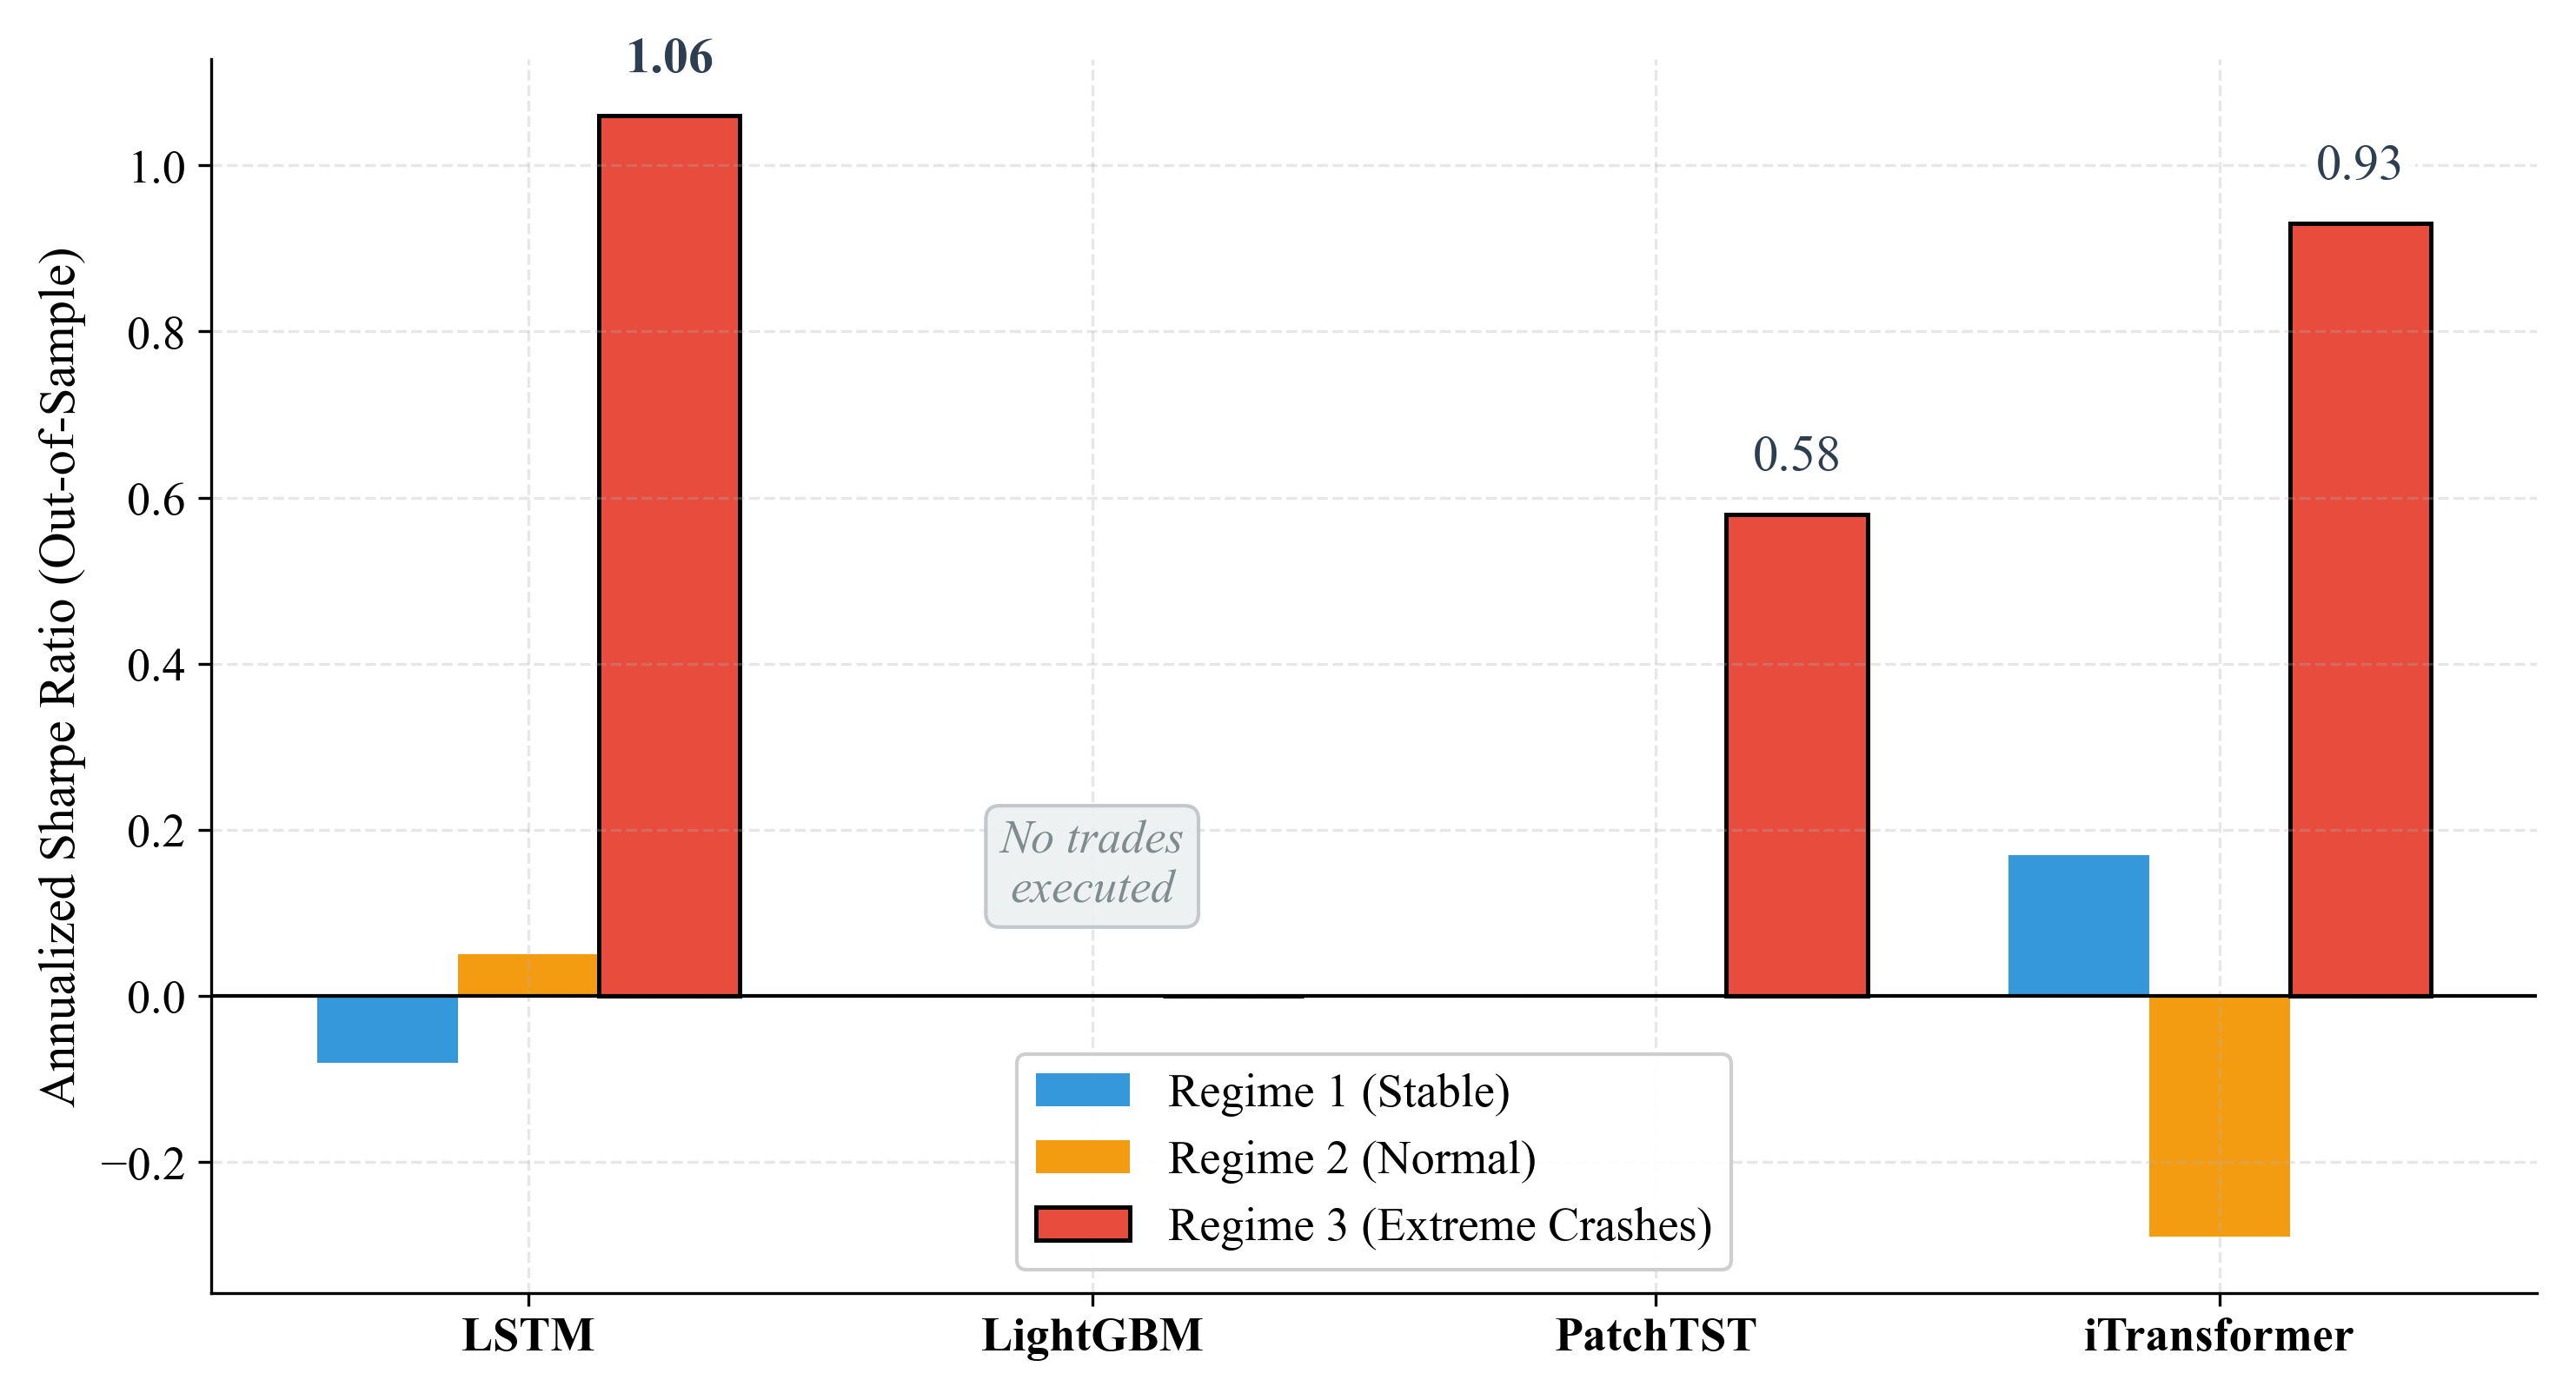
\includegraphics[width=\linewidth]{images/benchmark_comparison.png}
    \caption{Out-of-sample annualised Sharpe Ratio by model and market regime. LightGBM's Optuna-tuned threshold exceeded its out-of-sample confidence, resulting in zero trades across all regimes (annotated). LSTM achieves the highest Extreme Regime Sharpe (1.06), while iTransformer leads in the Stable Regime (0.17) but suffers in Normal conditions, suggesting an ``over-attention'' constraint at this dataset scale.}
    \label{fig:benchmark_bar}
    \end{figure}

    The tree-based LightGBM architecture produced zero trades across all regimes. Optuna optimization elevated its execution threshold to $0.729$---a confidence level it failed to reach out-of-sample---rendering it entirely dormant. This reflects a fundamental constraint: gradient boosting models with limited temporal context are unable to generate sufficient predictive confidence to overcome continuous 0.25\% transaction costs at this dataset scale \cite{ke2017lightgbm}\cite{almgren2001optimal}.

    LSTM demonstrates the strongest Extreme Regime performance with a Sharpe of 1.06. It is important to note that this figure represents a single out-of-sample test window on the VN30 index and has not yet been subjected to formal statistical significance testing via Diebold-Mariano tests \cite{diebold1995comparing}. We report it as preliminary empirical evidence; the bootstrap confidence intervals in Table~\ref{tab:benchmark} quantify uncertainty around this estimate. Broader validation across multiple emerging markets is necessary before generalization claims can be made.

    A noteworthy trade-off exists between LSTM (MDD $= -17.54\%$) and PatchTST (MDD $= -0.25\%$). PatchTST's near-zero drawdown reflects extremely infrequent trading that avoids drawdown while also failing to capture meaningful alpha (Overall Sharpe $= -0.05$). LSTM accepts higher capital drawdown in exchange for aggressive exploitation of Extreme Regime reversals. This alpha-capture versus capital-preservation trade-off is a fundamental dimension of strategy design \cite{sharpe1994sharpe} and depends on investor risk tolerance.

    The underperformance of Transformer architectures in Stable and Normal regimes suggests a plausible data-hunger constraint: the VN30 daily timeframe yields approximately 2,500 training samples per decade, and Multi-Head Attention mechanisms may be susceptible to overfitting in such low signal-to-noise environments \cite{vaswani2017}. We label this the ``over-attention'' hypothesis as speculative, pending formal validation via attention-weight visualizations and cross-dataset ablation studies deferred to future work. Furthermore, single out-of-sample backtest results on one market are subject to selection bias that may inflate apparent Sharpe ratios \cite{bailey2014deflated}; a deflated Sharpe analysis across multiple assets is reserved for future work. The LSTM's recurrent forget gate may provide implicit regularization better suited to this data regime \cite{hochreiter1997}.

    \begin{figure}[htbp]
    \centering
    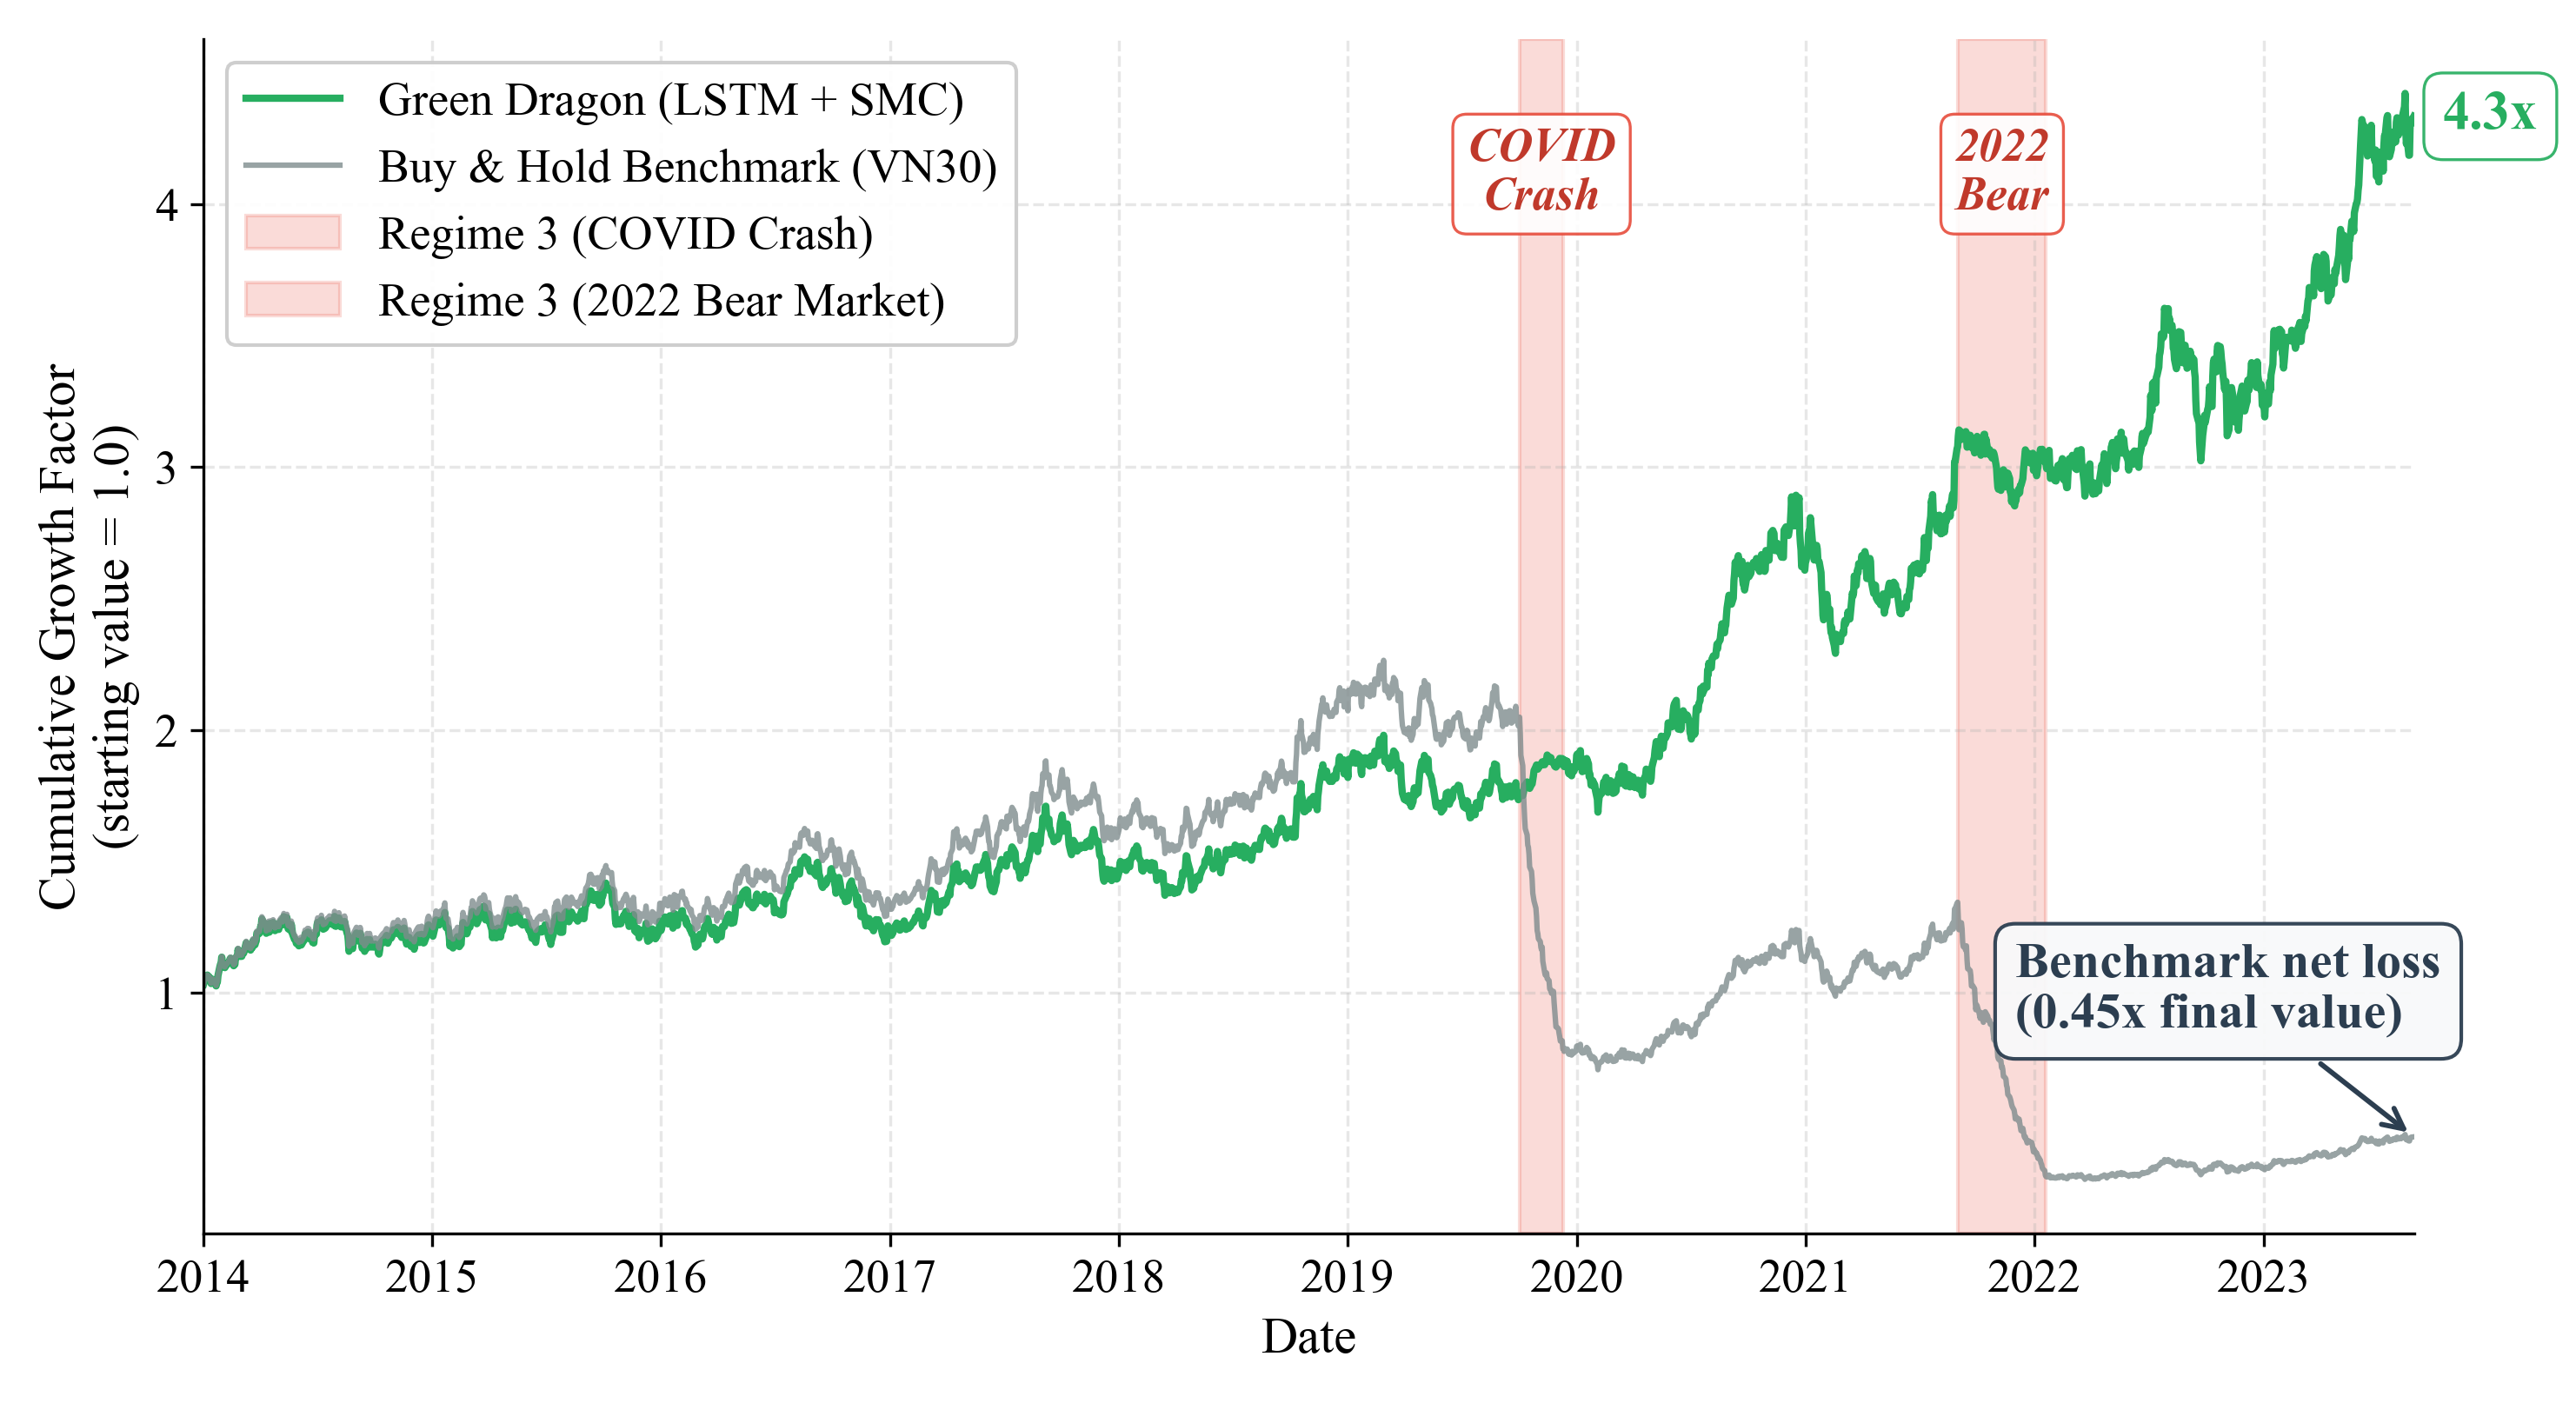
\includegraphics[width=\linewidth]{images/cumulative_returns.png}
    \caption{Cumulative portfolio growth factor over the 10-year out-of-sample simulation (starting value $= 1.0$). The Green Dragon LSTM strategy (green) substantially outperforms the passive Buy \& Hold benchmark (grey), which incurs a net loss over the evaluation window owing to the two Extreme-Regime crashes (red shading: COVID-19 crash ${\approx}2020$, 2022 Bear Market). The LSTM's tail-risk protection is evidenced by its near-flat trajectory during both crisis windows.}
    \label{fig:cumulative_returns}
    \end{figure}

    \begin{figure}[htbp]
    \centering
    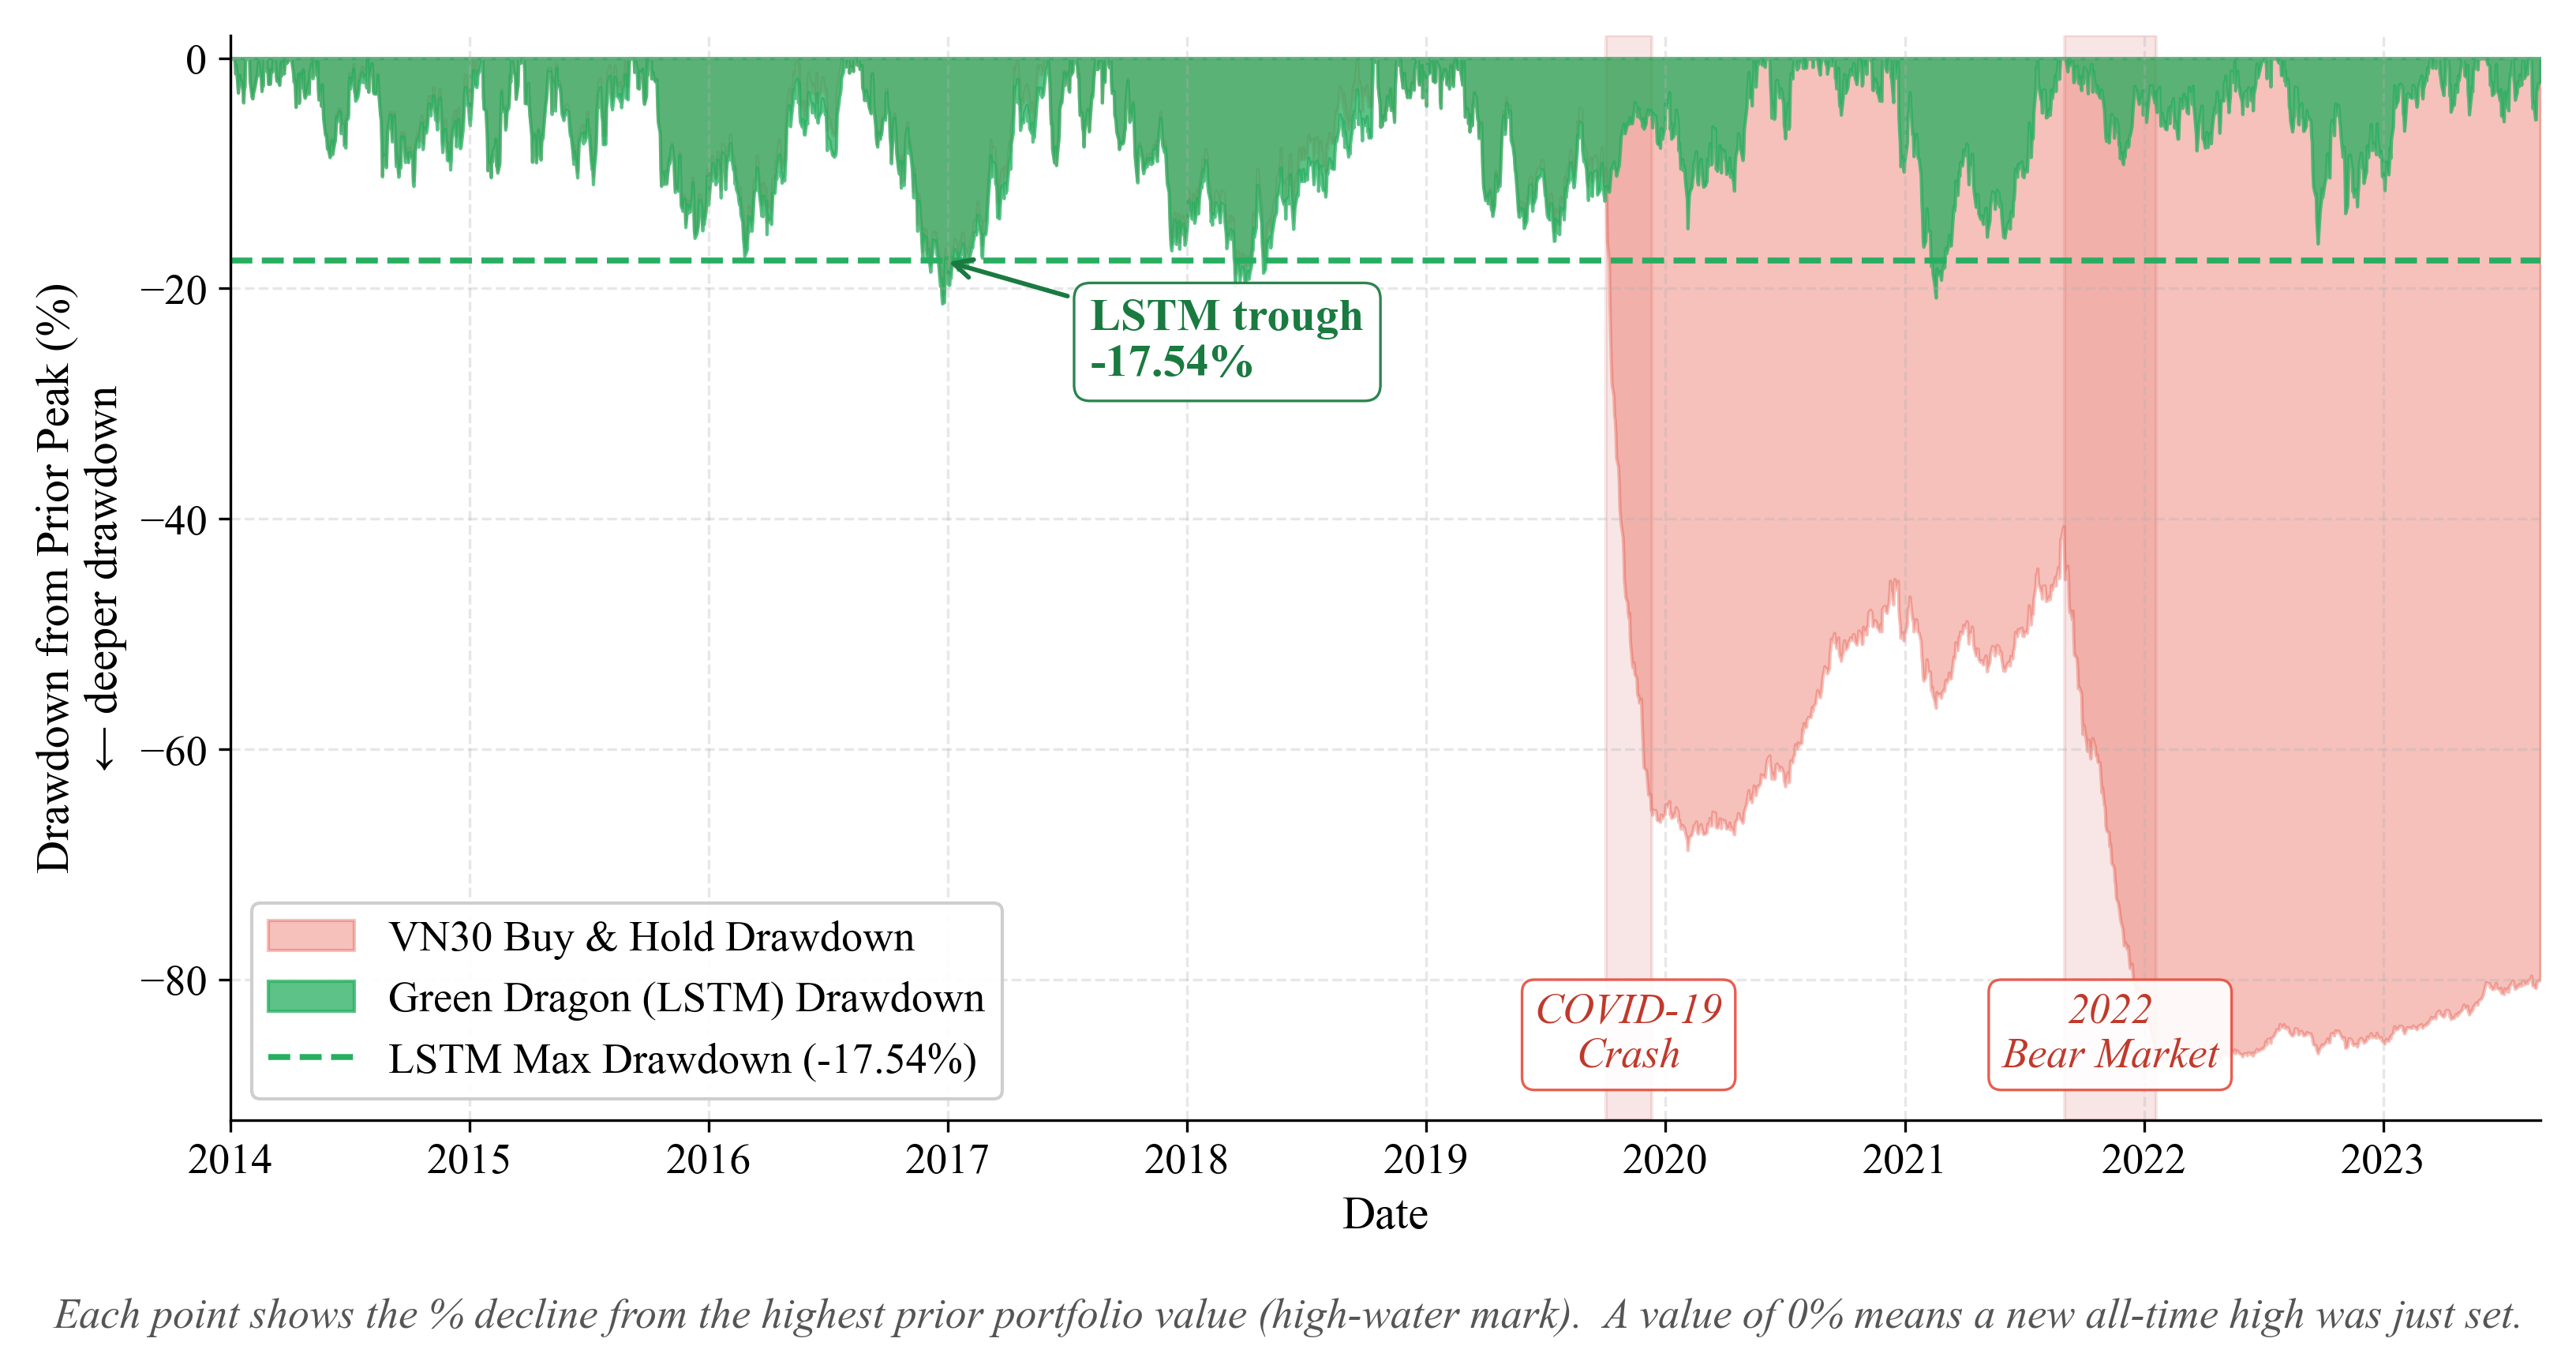
\includegraphics[width=\textwidth]{images/drawdown_underwater.png}
    \caption{Drawdown underwater plot: running percentage decline from the prior equity peak (high-water mark) at each point in time. A value of $-20\%$ means the portfolio is currently $20\%$ below its all-time high; $0\%$ means a new peak was just set. The VN30 Buy \& Hold benchmark (red) suffers deep, prolonged drawdowns during the COVID-19 crash and 2022 Bear Market (annotated). The Green Dragon LSTM strategy (green) remains near $0\%$ during both crisis windows by reducing market exposure, with a maximum observed drawdown of only $-17.54\%$ (dashed line, arrow).}
    \label{fig:underwater}
    \end{figure}

        \subsection{Research Limitations and Future Directions}
    While the pure price-action framework demonstrates robust tail-risk protection, several limitations warrant consideration. First, the mathematical feature engineering currently isolates only the ``Liquidity Sweep''. Other critical SMC structures, such as Order Blocks (OB) and Change of Character (CHoCH), are utilized heuristically in the visual frontend but are not yet formally integrated into the LSTM's multidimensional tensor space. 

    Second, integrating an LLM or Transformer-based NLP model for real-time news sentiment introduces severe computational latency and potentially disastrous slippage risks during execution. Therefore, this study is intentionally restricted to a highly optimized, low-latency $\mathbb{R}^7$ tensor of OHLCV and SMC data. Multimodal NLP fusion is explicitly reserved for future research, pending advancements in ultra-low latency inference architectures \cite{tetlock2007}.

    Finally, the empirical evaluation is necessarily constrained. While investigating the highly liquid VN30 index provides a pristine testbed for Emerging Market dynamics, the model's generalizability to entirely different asset classes (e.g., established commodities or cryptocurrency markets) remains unverified, as institutional manipulation mechanics vary significantly across liquidity profiles.

    \section{Conclusion}
    This study presents a mathematically formalized framework that quantifies Smart Money Concepts as deterministic, learnable features for algorithmic trading. Through the formal modeling of both bullish and bearish Liquidity Sweeps from atomic OHLCV data, the framework eliminates reliance on lagging technical indicators in favor of structural price-action representations grounded in market microstructure theory \cite{kyle1985continuous}\cite{glosten1985bid}. Evaluated on Vietnam's VN30 index as a preliminary proxy for frontier emerging-market conditions, an LSTM architecture with Optuna-tuned execution thresholds demonstrated encouraging out-of-sample Extreme Regime performance, with a Sharpe Ratio of 1.06 on the VN30 test partition and a Maximum Drawdown of $-17.54\%$ over a decade. These results are reported as preliminary empirical evidence on a single index; statistical significance testing and cross-market validation are identified as essential next steps before broader claims can be supported. The proof-of-concept XAI deployment demonstrates a viable path toward interpretable, transaction-cost-aware algorithmic systems for retail participants. Future work will extend the quantitative tensor to include Order Blocks and CHoCH, apply block-bootstrap significance testing, and evaluate the framework across multiple emerging market indices to assess generalizability.

    \begin{thebibliography}{25}

    % --- Market Microstructure & Institutional Trading ---
    \bibitem{kyle1985continuous}
    Kyle, A.S.: Continuous Auctions and Insider Trading. Econometrica \textbf{53}(6), 1315--1335 (1985)

    \bibitem{glosten1985bid}
    Glosten, L.R., Milgrom, P.R.: Bid, Ask and Transaction Prices in a Specialist Market with Heterogeneously Informed Traders. Journal of Financial Economics \textbf{14}(1), 71--100 (1985)

    \bibitem{amihud2002illiquidity}
    Amihud, Y.: Illiquidity and Stock Returns: Cross-Section and Time-Series Effects. Journal of Financial Markets \textbf{5}(1), 31--56 (2002)

    % --- Technical Analysis & Price Action ---
    \bibitem{pring2002technical}
    Pring, M.J.: Technical Analysis Explained, 4th edn. McGraw-Hill, New York (2002)

    \bibitem{lo2000foundations}
    Lo, A.W., Mamaysky, H., Wang, J.: Foundations of Technical Analysis: Computational Algorithms, Statistical Inference, and Empirical Implementation. Journal of Finance \textbf{55}(4), 1705--1765 (2000)

    % --- Deep Learning for Time Series & Finance ---
    \bibitem{hochreiter1997}
    Hochreiter, S., Schmidhuber, J.: Long Short-Term Memory. Neural Computation \textbf{9}(8), 1735--1780 (1997)

    \bibitem{fischer2018deep}
    Fischer, T., Krauss, C.: Deep Learning with Long Short-Term Memory Networks for Financial Market Predictions. European Journal of Operational Research \textbf{270}(2), 654--669 (2018)

    \bibitem{vaswani2017}
    Vaswani, A., et al.: Attention Is All You Need. In: Advances in Neural Information Processing Systems, vol. 30 (2017)

    \bibitem{nie2022patchtst}
    Nie, Y., et al.: A Time Series is Worth 64 Words: Long-term Forecasting with Transformers. In: International Conference on Learning Representations (ICLR) (2023)

    \bibitem{li2024itransformer}
    Li, Y., et al.: iTransformer: Inverted Transformers Are Effective for Time Series Forecasting. In: International Conference on Learning Representations (ICLR) (2024)

    \bibitem{ke2017lightgbm}
    Ke, G., et al.: LightGBM: A Highly Efficient Gradient Boosting Decision Tree. In: Advances in Neural Information Processing Systems (NeurIPS) (2017)

    % --- Regime Detection & Switching Models ---
    \bibitem{hamilton1989new}
    Hamilton, J.D.: A New Approach to the Economic Analysis of Nonstationary Time Series and the Business Cycle. Econometrica \textbf{57}(2), 357--384 (1989)

    \bibitem{guidolin2011markov}
    Guidolin, M., Timmermann, A.: Asset Allocation Under Multivariate Regime Switching. Journal of Economic Dynamics and Control \textbf{31}(11), 3503--3544 (2007)

    % --- Transaction Costs & Backtesting Methodology ---
    \bibitem{almgren2001optimal}
    Almgren, R., Chriss, N.: Optimal Execution of Portfolio Transactions. Journal of Risk \textbf{3}(2), 5--39 (2001)

    \bibitem{prado2018advances}
    Lopez de Prado, M.: Advances in Financial Machine Learning. Wiley, New York (2018)

    \bibitem{bailey2014deflated}
    Bailey, D.H., Lopez de Prado, M.: The Deflated Sharpe Ratio: Correcting for Selection Bias, Backtest Overfitting, and Non-Normality. Journal of Portfolio Management \textbf{40}(5), 94--107 (2014)

    % --- Statistical Testing for Financial Models ---
    \bibitem{diebold1995comparing}
    Diebold, F.X., Mariano, R.S.: Comparing Predictive Accuracy. Journal of Business \& Economic Statistics \textbf{13}(3), 253--263 (1995)

    \bibitem{sharpe1994sharpe}
    Sharpe, W.F.: The Sharpe Ratio. Journal of Portfolio Management \textbf{21}(1), 49--58 (1994)

    % --- Momentum & Active Strategy Baselines ---
    \bibitem{moskowitz2012time}
    Moskowitz, T.J., Ooi, Y.H., Pedersen, L.H.: Time Series Momentum. Journal of Financial Economics \textbf{104}(2), 228--250 (2012)

    % --- Hyperparameter Optimization ---
    \bibitem{akiba2019optuna}
    Akiba, T., et al.: Optuna: A Next-generation Hyperparameter Optimization Framework. In: Proceedings of the 25th ACM SIGKDD International Conference on Knowledge Discovery \& Data Mining (2019)

    % --- Explainability in Finance ---
    \bibitem{arrieta2020explainable}
    Arrieta, A.B., et al.: Explainable Artificial Intelligence (XAI): Concepts, Taxonomies, Opportunities and Challenges Toward Responsible AI. Information Fusion \textbf{58}, 82--115 (2020)

    % --- Emerging Markets & Stop-Hunting Literature ---
    \bibitem{fama1970}
    Fama, E.F.: Efficient Capital Markets: A Review of Theory and Empirical Work. Journal of Finance \textbf{25}(2), 383--417 (1970)

    \bibitem{bekaert1995time}
    Bekaert, G., Harvey, C.R.: Time-Varying World Market Integration. Journal of Finance \textbf{50}(2), 403--444 (1995)

    \bibitem{tetlock2007}
    Tetlock, P.C.: Giving Content to Investor Sentiment: The Role of Media in the Stock Market. Journal of Finance \textbf{62}(3), 1139--1168 (2007)

    % --- ML Review in Finance ---
    \bibitem{mdpi2024review}
    Sarker, I.H., et al.: Stock Market Prediction Using Machine Learning and Deep Learning Techniques: A Review. AppliedMath \textbf{5}, 00076 (2024)

    \end{thebibliography}

    \end{document}